% Created by tikzDevice version 0.7.0 on 2014-06-29 19:48:02
% !TEX encoding = UTF-8 Unicode
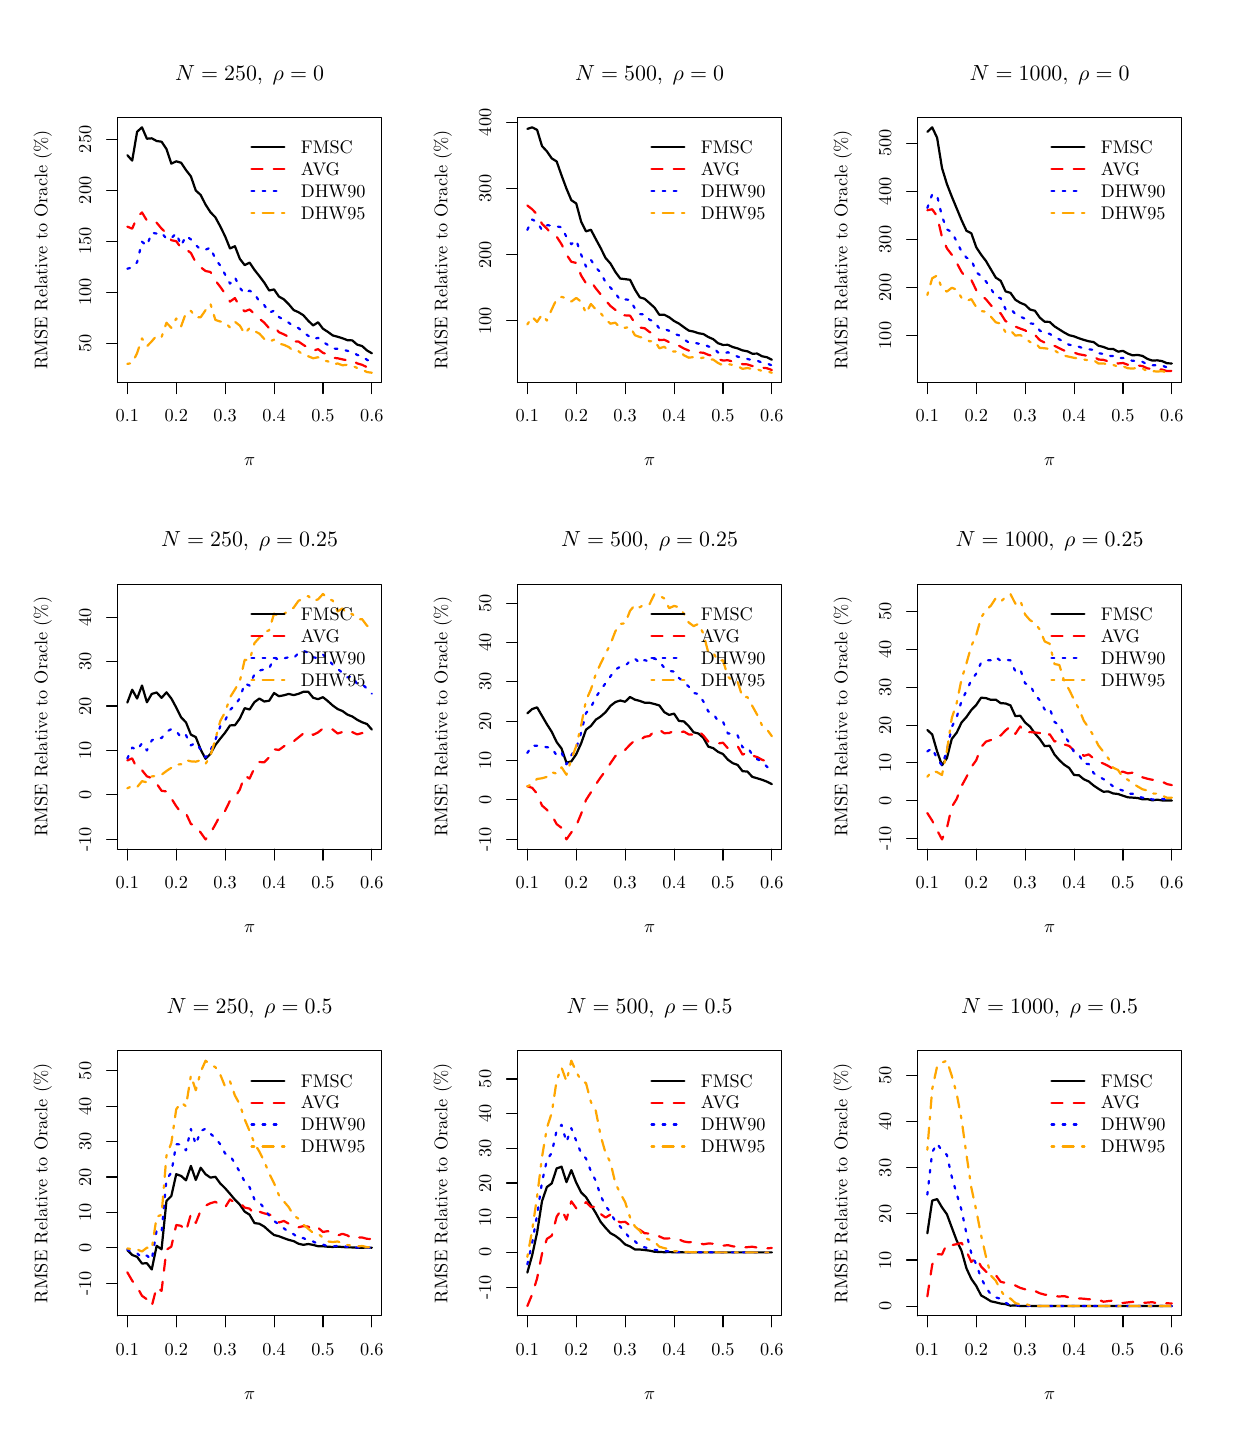
\begin{tikzpicture}[x=1pt,y=1pt]
\definecolor[named]{fillColor}{rgb}{1.00,1.00,1.00}
\path[use as bounding box,fill=fillColor,fill opacity=0.00] (0,0) rectangle (433.62,505.89);
\begin{scope}
\path[clip] ( 32.47,377.65) rectangle (127.91,473.42);
\definecolor[named]{drawColor}{rgb}{0.00,0.00,0.00}

\path[draw=drawColor,line width= 0.8pt,line join=round,line cap=round] ( 36.01,459.81) --
	( 37.77,457.84) --
	( 39.54,468.27) --
	( 41.31,469.87) --
	( 43.08,465.76) --
	( 44.84,465.90) --
	( 46.61,464.93) --
	( 48.38,464.68) --
	( 50.15,462.02) --
	( 51.91,456.74) --
	( 53.68,457.60) --
	( 55.45,457.07) --
	( 57.21,454.43) --
	( 58.98,452.15) --
	( 60.75,447.04) --
	( 62.52,445.43) --
	( 64.28,441.95) --
	( 66.05,439.20) --
	( 67.82,437.37) --
	( 69.59,434.08) --
	( 71.35,430.48) --
	( 73.12,426.10) --
	( 74.89,426.92) --
	( 76.66,422.36) --
	( 78.42,420.08) --
	( 80.19,421.00) --
	( 81.96,418.34) --
	( 83.72,416.13) --
	( 85.49,413.77) --
	( 87.26,410.92) --
	( 89.03,411.30) --
	( 90.79,408.72) --
	( 92.56,407.73) --
	( 94.33,405.97) --
	( 96.10,403.84) --
	( 97.86,403.07) --
	( 99.63,401.96) --
	(101.40,399.96) --
	(103.17,398.29) --
	(104.93,399.43) --
	(106.70,397.10) --
	(108.47,395.96) --
	(110.23,394.68) --
	(112.00,394.20) --
	(113.77,393.65) --
	(115.54,392.96) --
	(117.30,392.88) --
	(119.07,391.35) --
	(120.84,390.85) --
	(122.61,389.25) --
	(124.37,388.22);
\end{scope}
\begin{scope}
\path[clip] (  0.00,  0.00) rectangle (433.62,505.89);
\definecolor[named]{drawColor}{rgb}{0.00,0.00,0.00}

\path[draw=drawColor,line width= 0.4pt,line join=round,line cap=round] ( 36.01,377.65) -- (124.37,377.65);

\path[draw=drawColor,line width= 0.4pt,line join=round,line cap=round] ( 36.01,377.65) -- ( 36.01,373.69);

\path[draw=drawColor,line width= 0.4pt,line join=round,line cap=round] ( 53.68,377.65) -- ( 53.68,373.69);

\path[draw=drawColor,line width= 0.4pt,line join=round,line cap=round] ( 71.35,377.65) -- ( 71.35,373.69);

\path[draw=drawColor,line width= 0.4pt,line join=round,line cap=round] ( 89.03,377.65) -- ( 89.03,373.69);

\path[draw=drawColor,line width= 0.4pt,line join=round,line cap=round] (106.70,377.65) -- (106.70,373.69);

\path[draw=drawColor,line width= 0.4pt,line join=round,line cap=round] (124.37,377.65) -- (124.37,373.69);

\node[text=drawColor,anchor=base,inner sep=0pt, outer sep=0pt, scale=  0.66] at ( 36.01,363.40) {0.1};

\node[text=drawColor,anchor=base,inner sep=0pt, outer sep=0pt, scale=  0.66] at ( 53.68,363.40) {0.2};

\node[text=drawColor,anchor=base,inner sep=0pt, outer sep=0pt, scale=  0.66] at ( 71.35,363.40) {0.3};

\node[text=drawColor,anchor=base,inner sep=0pt, outer sep=0pt, scale=  0.66] at ( 89.03,363.40) {0.4};

\node[text=drawColor,anchor=base,inner sep=0pt, outer sep=0pt, scale=  0.66] at (106.70,363.40) {0.5};

\node[text=drawColor,anchor=base,inner sep=0pt, outer sep=0pt, scale=  0.66] at (124.37,363.40) {0.6};

\path[draw=drawColor,line width= 0.4pt,line join=round,line cap=round] ( 32.47,391.87) -- ( 32.47,465.53);

\path[draw=drawColor,line width= 0.4pt,line join=round,line cap=round] ( 32.47,391.87) -- ( 28.51,391.87);

\path[draw=drawColor,line width= 0.4pt,line join=round,line cap=round] ( 32.47,410.28) -- ( 28.51,410.28);

\path[draw=drawColor,line width= 0.4pt,line join=round,line cap=round] ( 32.47,428.70) -- ( 28.51,428.70);

\path[draw=drawColor,line width= 0.4pt,line join=round,line cap=round] ( 32.47,447.12) -- ( 28.51,447.12);

\path[draw=drawColor,line width= 0.4pt,line join=round,line cap=round] ( 32.47,465.53) -- ( 28.51,465.53);

\node[text=drawColor,rotate= 90.00,anchor=base,inner sep=0pt, outer sep=0pt, scale=  0.66] at ( 22.97,391.87) {50};

\node[text=drawColor,rotate= 90.00,anchor=base,inner sep=0pt, outer sep=0pt, scale=  0.66] at ( 22.97,410.28) {100};

\node[text=drawColor,rotate= 90.00,anchor=base,inner sep=0pt, outer sep=0pt, scale=  0.66] at ( 22.97,428.70) {150};

\node[text=drawColor,rotate= 90.00,anchor=base,inner sep=0pt, outer sep=0pt, scale=  0.66] at ( 22.97,447.12) {200};

\node[text=drawColor,rotate= 90.00,anchor=base,inner sep=0pt, outer sep=0pt, scale=  0.66] at ( 22.97,465.53) {250};

\path[draw=drawColor,line width= 0.4pt,line join=round,line cap=round] ( 32.47,377.65) --
	(127.91,377.65) --
	(127.91,473.42) --
	( 32.47,473.42) --
	( 32.47,377.65);
\end{scope}
\begin{scope}
\path[clip] (  0.00,337.26) rectangle (144.54,505.89);
\definecolor[named]{drawColor}{rgb}{0.00,0.00,0.00}

\node[text=drawColor,anchor=base,inner sep=0pt, outer sep=0pt, scale=  0.79] at ( 80.19,486.92) {\bfseries $N=250, \;\rho=0$};

\node[text=drawColor,anchor=base,inner sep=0pt, outer sep=0pt, scale=  0.66] at ( 80.19,347.56) {$\pi$};

\node[text=drawColor,rotate= 90.00,anchor=base,inner sep=0pt, outer sep=0pt, scale=  0.66] at (  7.13,425.53) {RMSE Relative to Oracle (\%)};
\end{scope}
\begin{scope}
\path[clip] ( 32.47,377.65) rectangle (127.91,473.42);
\definecolor[named]{drawColor}{rgb}{1.00,0.00,0.00}

\path[draw=drawColor,line width= 0.8pt,dash pattern=on 4pt off 4pt ,line join=round,line cap=round] ( 36.01,433.99) --
	( 37.77,433.25) --
	( 39.54,437.44) --
	( 41.31,439.12) --
	( 43.08,436.19) --
	( 44.84,435.35) --
	( 46.61,435.40) --
	( 48.38,433.27) --
	( 50.15,431.62) --
	( 51.91,429.08) --
	( 53.68,428.73) --
	( 55.45,426.26) --
	( 57.21,425.77) --
	( 58.98,424.48) --
	( 60.75,421.03) --
	( 62.52,419.29) --
	( 64.28,417.96) --
	( 66.05,417.59) --
	( 67.82,414.52) --
	( 69.59,412.24) --
	( 71.35,409.74) --
	( 73.12,406.91) --
	( 74.89,408.18) --
	( 76.66,405.00) --
	( 78.42,403.37) --
	( 80.19,404.06) --
	( 81.96,402.45) --
	( 83.72,400.74) --
	( 85.49,399.29) --
	( 87.26,397.27) --
	( 89.03,397.87) --
	( 90.79,395.85) --
	( 92.56,395.08) --
	( 94.33,394.13) --
	( 96.10,392.45) --
	( 97.86,392.47) --
	( 99.63,391.24) --
	(101.40,390.16) --
	(103.17,389.19) --
	(104.93,389.71) --
	(106.70,388.40) --
	(108.47,387.76) --
	(110.23,386.59) --
	(112.00,386.42) --
	(113.77,386.02) --
	(115.54,385.67) --
	(117.30,385.70) --
	(119.07,384.57) --
	(120.84,384.06) --
	(122.61,383.20) --
	(124.37,382.45);
\definecolor[named]{drawColor}{rgb}{0.00,0.00,1.00}

\path[draw=drawColor,line width= 0.8pt,dash pattern=on 1pt off 3pt ,line join=round,line cap=round] ( 36.01,418.78) --
	( 37.77,419.24) --
	( 39.54,421.11) --
	( 41.31,428.52) --
	( 43.08,427.12) --
	( 44.84,431.79) --
	( 46.61,431.48) --
	( 48.38,431.83) --
	( 50.15,429.60) --
	( 51.91,429.82) --
	( 53.68,431.60) --
	( 55.45,427.16) --
	( 57.21,430.67) --
	( 58.98,429.37) --
	( 60.75,427.36) --
	( 62.52,425.68) --
	( 64.28,425.64) --
	( 66.05,426.43) --
	( 67.82,422.28) --
	( 69.59,419.93) --
	( 71.35,416.66) --
	( 73.12,413.40) --
	( 74.89,415.69) --
	( 76.66,411.85) --
	( 78.42,409.83) --
	( 80.19,410.86) --
	( 81.96,409.80) --
	( 83.72,406.88) --
	( 85.49,405.61) --
	( 87.26,402.91) --
	( 89.03,403.61) --
	( 90.79,401.34) --
	( 92.56,400.27) --
	( 94.33,399.27) --
	( 96.10,398.00) --
	( 97.86,397.33) --
	( 99.63,395.79) --
	(101.40,394.53) --
	(103.17,393.35) --
	(104.93,393.81) --
	(106.70,392.30) --
	(108.47,391.26) --
	(110.23,389.97) --
	(112.00,389.83) --
	(113.77,389.62) --
	(115.54,389.10) --
	(117.30,388.72) --
	(119.07,387.62) --
	(120.84,387.17) --
	(122.61,385.88) --
	(124.37,384.90);
\definecolor[named]{drawColor}{rgb}{1.00,0.65,0.00}

\path[draw=drawColor,line width= 0.8pt,dash pattern=on 1pt off 3pt on 4pt off 3pt ,line join=round,line cap=round] ( 36.01,384.39) --
	( 37.77,384.71) --
	( 39.54,388.29) --
	( 41.31,393.61) --
	( 43.08,390.72) --
	( 44.84,392.56) --
	( 46.61,394.61) --
	( 48.38,394.08) --
	( 50.15,399.26) --
	( 51.91,397.42) --
	( 53.68,400.79) --
	( 55.45,397.97) --
	( 57.21,402.86) --
	( 58.98,403.57) --
	( 60.75,401.21) --
	( 62.52,401.25) --
	( 64.28,403.82) --
	( 66.05,406.07) --
	( 67.82,400.30) --
	( 69.59,399.70) --
	( 71.35,399.39) --
	( 73.12,397.52) --
	( 74.89,399.60) --
	( 76.66,398.23) --
	( 78.42,395.26) --
	( 80.19,397.38) --
	( 81.96,396.25) --
	( 83.72,395.34) --
	( 85.49,393.42) --
	( 87.26,392.41) --
	( 89.03,393.15) --
	( 90.79,391.73) --
	( 92.56,391.29) --
	( 94.33,390.48) --
	( 96.10,389.02) --
	( 97.86,388.98) --
	( 99.63,387.63) --
	(101.40,387.14) --
	(103.17,386.43) --
	(104.93,386.79) --
	(106.70,385.57) --
	(108.47,385.34) --
	(110.23,384.18) --
	(112.00,384.54) --
	(113.77,383.89) --
	(115.54,384.07) --
	(117.30,383.75) --
	(119.07,382.89) --
	(120.84,382.32) --
	(122.61,381.44) --
	(124.37,381.20);
\definecolor[named]{drawColor}{rgb}{0.00,0.00,0.00}

\path[draw=drawColor,line width= 0.8pt,line join=round,line cap=round] ( 80.89,462.63) -- ( 92.77,462.63);
\definecolor[named]{drawColor}{rgb}{1.00,0.00,0.00}

\path[draw=drawColor,line width= 0.8pt,dash pattern=on 4pt off 4pt ,line join=round,line cap=round] ( 80.89,454.71) -- ( 92.77,454.71);
\definecolor[named]{drawColor}{rgb}{0.00,0.00,1.00}

\path[draw=drawColor,line width= 0.8pt,dash pattern=on 1pt off 3pt ,line join=round,line cap=round] ( 80.89,446.79) -- ( 92.77,446.79);
\definecolor[named]{drawColor}{rgb}{1.00,0.65,0.00}

\path[draw=drawColor,line width= 0.8pt,dash pattern=on 1pt off 3pt on 4pt off 3pt ,line join=round,line cap=round] ( 80.89,438.87) -- ( 92.77,438.87);
\definecolor[named]{drawColor}{rgb}{0.00,0.00,0.00}

\node[text=drawColor,anchor=base west,inner sep=0pt, outer sep=0pt, scale=  0.66] at ( 98.71,460.35) {FMSC};

\node[text=drawColor,anchor=base west,inner sep=0pt, outer sep=0pt, scale=  0.66] at ( 98.71,452.43) {AVG};

\node[text=drawColor,anchor=base west,inner sep=0pt, outer sep=0pt, scale=  0.66] at ( 98.71,444.51) {DHW90};

\node[text=drawColor,anchor=base west,inner sep=0pt, outer sep=0pt, scale=  0.66] at ( 98.71,436.59) {DHW95};
\end{scope}
\begin{scope}
\path[clip] (177.01,377.65) rectangle (272.45,473.42);
\definecolor[named]{drawColor}{rgb}{0.00,0.00,0.00}

\path[draw=drawColor,line width= 0.8pt,line join=round,line cap=round] (180.55,469.31) --
	(182.31,469.87) --
	(184.08,468.96) --
	(185.85,463.11) --
	(187.62,461.19) --
	(189.38,458.64) --
	(191.15,457.54) --
	(192.92,452.49) --
	(194.69,447.73) --
	(196.45,443.54) --
	(198.22,442.36) --
	(199.99,435.81) --
	(201.75,432.27) --
	(203.52,432.86) --
	(205.29,429.50) --
	(207.06,426.23) --
	(208.82,422.66) --
	(210.59,420.66) --
	(212.36,417.63) --
	(214.13,415.23) --
	(215.89,415.02) --
	(217.66,414.78) --
	(219.43,411.25) --
	(221.20,408.45) --
	(222.96,407.89) --
	(224.73,406.33) --
	(226.50,404.74) --
	(228.26,402.13) --
	(230.03,402.15) --
	(231.80,401.25) --
	(233.57,399.89) --
	(235.33,398.97) --
	(237.10,397.66) --
	(238.87,396.43) --
	(240.64,396.07) --
	(242.40,395.47) --
	(244.17,395.18) --
	(245.94,394.10) --
	(247.71,393.33) --
	(249.47,391.85) --
	(251.24,391.25) --
	(253.01,391.28) --
	(254.77,390.48) --
	(256.54,389.99) --
	(258.31,389.27) --
	(260.08,388.94) --
	(261.84,388.07) --
	(263.61,388.12) --
	(265.38,387.15) --
	(267.15,386.79) --
	(268.91,385.90);
\end{scope}
\begin{scope}
\path[clip] (  0.00,  0.00) rectangle (433.62,505.89);
\definecolor[named]{drawColor}{rgb}{0.00,0.00,0.00}

\path[draw=drawColor,line width= 0.4pt,line join=round,line cap=round] (180.55,377.65) -- (268.91,377.65);

\path[draw=drawColor,line width= 0.4pt,line join=round,line cap=round] (180.55,377.65) -- (180.55,373.69);

\path[draw=drawColor,line width= 0.4pt,line join=round,line cap=round] (198.22,377.65) -- (198.22,373.69);

\path[draw=drawColor,line width= 0.4pt,line join=round,line cap=round] (215.89,377.65) -- (215.89,373.69);

\path[draw=drawColor,line width= 0.4pt,line join=round,line cap=round] (233.57,377.65) -- (233.57,373.69);

\path[draw=drawColor,line width= 0.4pt,line join=round,line cap=round] (251.24,377.65) -- (251.24,373.69);

\path[draw=drawColor,line width= 0.4pt,line join=round,line cap=round] (268.91,377.65) -- (268.91,373.69);

\node[text=drawColor,anchor=base,inner sep=0pt, outer sep=0pt, scale=  0.66] at (180.55,363.40) {0.1};

\node[text=drawColor,anchor=base,inner sep=0pt, outer sep=0pt, scale=  0.66] at (198.22,363.40) {0.2};

\node[text=drawColor,anchor=base,inner sep=0pt, outer sep=0pt, scale=  0.66] at (215.89,363.40) {0.3};

\node[text=drawColor,anchor=base,inner sep=0pt, outer sep=0pt, scale=  0.66] at (233.57,363.40) {0.4};

\node[text=drawColor,anchor=base,inner sep=0pt, outer sep=0pt, scale=  0.66] at (251.24,363.40) {0.5};

\node[text=drawColor,anchor=base,inner sep=0pt, outer sep=0pt, scale=  0.66] at (268.91,363.40) {0.6};

\path[draw=drawColor,line width= 0.4pt,line join=round,line cap=round] (177.01,400.02) -- (177.01,471.66);

\path[draw=drawColor,line width= 0.4pt,line join=round,line cap=round] (177.01,400.02) -- (173.05,400.02);

\path[draw=drawColor,line width= 0.4pt,line join=round,line cap=round] (177.01,423.90) -- (173.05,423.90);

\path[draw=drawColor,line width= 0.4pt,line join=round,line cap=round] (177.01,447.78) -- (173.05,447.78);

\path[draw=drawColor,line width= 0.4pt,line join=round,line cap=round] (177.01,471.66) -- (173.05,471.66);

\node[text=drawColor,rotate= 90.00,anchor=base,inner sep=0pt, outer sep=0pt, scale=  0.66] at (167.51,400.02) {100};

\node[text=drawColor,rotate= 90.00,anchor=base,inner sep=0pt, outer sep=0pt, scale=  0.66] at (167.51,423.90) {200};

\node[text=drawColor,rotate= 90.00,anchor=base,inner sep=0pt, outer sep=0pt, scale=  0.66] at (167.51,447.78) {300};

\node[text=drawColor,rotate= 90.00,anchor=base,inner sep=0pt, outer sep=0pt, scale=  0.66] at (167.51,471.66) {400};

\path[draw=drawColor,line width= 0.4pt,line join=round,line cap=round] (177.01,377.65) --
	(272.45,377.65) --
	(272.45,473.42) --
	(177.01,473.42) --
	(177.01,377.65);
\end{scope}
\begin{scope}
\path[clip] (144.54,337.26) rectangle (289.08,505.89);
\definecolor[named]{drawColor}{rgb}{0.00,0.00,0.00}

\node[text=drawColor,anchor=base,inner sep=0pt, outer sep=0pt, scale=  0.79] at (224.73,486.92) {\bfseries $N=500, \;\rho=0$};

\node[text=drawColor,anchor=base,inner sep=0pt, outer sep=0pt, scale=  0.66] at (224.73,347.56) {$\pi$};

\node[text=drawColor,rotate= 90.00,anchor=base,inner sep=0pt, outer sep=0pt, scale=  0.66] at (151.67,425.53) {RMSE Relative to Oracle (\%)};
\end{scope}
\begin{scope}
\path[clip] (177.01,377.65) rectangle (272.45,473.42);
\definecolor[named]{drawColor}{rgb}{1.00,0.00,0.00}

\path[draw=drawColor,line width= 0.8pt,dash pattern=on 4pt off 4pt ,line join=round,line cap=round] (180.55,441.63) --
	(182.31,440.26) --
	(184.08,438.38) --
	(185.85,435.00) --
	(187.62,433.29) --
	(189.38,431.16) --
	(191.15,430.36) --
	(192.92,427.62) --
	(194.69,423.89) --
	(196.45,421.29) --
	(198.22,420.88) --
	(199.99,416.33) --
	(201.75,413.52) --
	(203.52,414.22) --
	(205.29,411.68) --
	(207.06,409.50) --
	(208.82,407.37) --
	(210.59,405.32) --
	(212.36,403.91) --
	(214.13,401.95) --
	(215.89,401.93) --
	(217.66,401.83) --
	(219.43,399.12) --
	(221.20,397.54) --
	(222.96,397.26) --
	(224.73,395.90) --
	(226.50,395.17) --
	(228.26,392.97) --
	(230.03,393.11) --
	(231.80,392.25) --
	(233.57,391.38) --
	(235.33,390.96) --
	(237.10,389.97) --
	(238.87,389.21) --
	(240.64,389.07) --
	(242.40,388.54) --
	(244.17,388.42) --
	(245.94,387.67) --
	(247.71,387.22) --
	(249.47,386.09) --
	(251.24,385.61) --
	(253.01,385.71) --
	(254.77,385.24) --
	(256.54,384.93) --
	(258.31,384.29) --
	(260.08,384.21) --
	(261.84,383.62) --
	(263.61,383.59) --
	(265.38,383.02) --
	(267.15,382.82) --
	(268.91,382.19);
\definecolor[named]{drawColor}{rgb}{0.00,0.00,1.00}

\path[draw=drawColor,line width= 0.8pt,dash pattern=on 1pt off 3pt ,line join=round,line cap=round] (180.55,432.81) --
	(182.31,436.56) --
	(184.08,435.62) --
	(185.85,432.76) --
	(187.62,434.50) --
	(189.38,434.37) --
	(191.15,434.06) --
	(192.92,433.78) --
	(194.69,430.27) --
	(196.45,427.64) --
	(198.22,429.05) --
	(199.99,423.90) --
	(201.75,419.55) --
	(203.52,422.01) --
	(205.29,419.15) --
	(207.06,417.43) --
	(208.82,413.83) --
	(210.59,411.94) --
	(212.36,410.03) --
	(214.13,407.38) --
	(215.89,407.68) --
	(217.66,407.53) --
	(219.43,404.40) --
	(221.20,402.38) --
	(222.96,402.32) --
	(224.73,400.34) --
	(226.50,399.64) --
	(228.26,397.14) --
	(230.03,396.96) --
	(231.80,396.36) --
	(233.57,395.23) --
	(235.33,394.73) --
	(237.10,393.32) --
	(238.87,392.12) --
	(240.64,392.08) --
	(242.40,391.71) --
	(244.17,391.56) --
	(245.94,390.69) --
	(247.71,390.22) --
	(249.47,388.51) --
	(251.24,388.06) --
	(253.01,388.60) --
	(254.77,387.81) --
	(256.54,387.01) --
	(258.31,386.57) --
	(260.08,386.17) --
	(261.84,385.75) --
	(263.61,385.56) --
	(265.38,384.82) --
	(267.15,384.55) --
	(268.91,383.83);
\definecolor[named]{drawColor}{rgb}{1.00,0.65,0.00}

\path[draw=drawColor,line width= 0.8pt,dash pattern=on 1pt off 3pt on 4pt off 3pt ,line join=round,line cap=round] (180.55,398.66) --
	(182.31,401.35) --
	(184.08,399.55) --
	(185.85,402.20) --
	(187.62,400.06) --
	(189.38,404.10) --
	(191.15,407.82) --
	(192.92,408.61) --
	(194.69,408.10) --
	(196.45,406.91) --
	(198.22,408.23) --
	(199.99,406.88) --
	(201.75,402.69) --
	(203.52,406.05) --
	(205.29,404.07) --
	(207.06,402.74) --
	(208.82,400.49) --
	(210.59,398.92) --
	(212.36,399.28) --
	(214.13,397.32) --
	(215.89,397.43) --
	(217.66,397.83) --
	(219.43,394.75) --
	(221.20,394.09) --
	(222.96,393.75) --
	(224.73,392.54) --
	(226.50,392.80) --
	(228.26,390.03) --
	(230.03,390.57) --
	(231.80,389.14) --
	(233.57,388.83) --
	(235.33,389.05) --
	(237.10,387.54) --
	(238.87,386.64) --
	(240.64,386.85) --
	(242.40,386.37) --
	(244.17,386.66) --
	(245.94,385.96) --
	(247.71,385.94) --
	(249.47,384.71) --
	(251.24,383.87) --
	(253.01,384.33) --
	(254.77,384.03) --
	(256.54,383.58) --
	(258.31,382.59) --
	(260.08,382.91) --
	(261.84,382.51) --
	(263.61,382.43) --
	(265.38,381.83) --
	(267.15,381.67) --
	(268.91,381.20);
\definecolor[named]{drawColor}{rgb}{0.00,0.00,0.00}

\path[draw=drawColor,line width= 0.8pt,line join=round,line cap=round] (225.43,462.63) -- (237.31,462.63);
\definecolor[named]{drawColor}{rgb}{1.00,0.00,0.00}

\path[draw=drawColor,line width= 0.8pt,dash pattern=on 4pt off 4pt ,line join=round,line cap=round] (225.43,454.71) -- (237.31,454.71);
\definecolor[named]{drawColor}{rgb}{0.00,0.00,1.00}

\path[draw=drawColor,line width= 0.8pt,dash pattern=on 1pt off 3pt ,line join=round,line cap=round] (225.43,446.79) -- (237.31,446.79);
\definecolor[named]{drawColor}{rgb}{1.00,0.65,0.00}

\path[draw=drawColor,line width= 0.8pt,dash pattern=on 1pt off 3pt on 4pt off 3pt ,line join=round,line cap=round] (225.43,438.87) -- (237.31,438.87);
\definecolor[named]{drawColor}{rgb}{0.00,0.00,0.00}

\node[text=drawColor,anchor=base west,inner sep=0pt, outer sep=0pt, scale=  0.66] at (243.25,460.35) {FMSC};

\node[text=drawColor,anchor=base west,inner sep=0pt, outer sep=0pt, scale=  0.66] at (243.25,452.43) {AVG};

\node[text=drawColor,anchor=base west,inner sep=0pt, outer sep=0pt, scale=  0.66] at (243.25,444.51) {DHW90};

\node[text=drawColor,anchor=base west,inner sep=0pt, outer sep=0pt, scale=  0.66] at (243.25,436.59) {DHW95};
\end{scope}
\begin{scope}
\path[clip] (321.55,377.65) rectangle (416.99,473.42);
\definecolor[named]{drawColor}{rgb}{0.00,0.00,0.00}

\path[draw=drawColor,line width= 0.8pt,line join=round,line cap=round] (325.09,468.21) --
	(326.85,469.87) --
	(328.62,466.10) --
	(330.39,455.18) --
	(332.16,449.38) --
	(333.92,444.86) --
	(335.69,440.59) --
	(337.46,436.32) --
	(339.23,432.49) --
	(340.99,431.58) --
	(342.76,426.55) --
	(344.53,423.85) --
	(346.29,421.55) --
	(348.06,418.53) --
	(349.83,415.56) --
	(351.60,414.41) --
	(353.36,410.59) --
	(355.13,410.06) --
	(356.90,407.56) --
	(358.67,406.47) --
	(360.43,405.73) --
	(362.20,404.04) --
	(363.97,403.59) --
	(365.74,401.09) --
	(367.50,399.61) --
	(369.27,399.57) --
	(371.04,397.95) --
	(372.80,396.83) --
	(374.57,395.72) --
	(376.34,394.76) --
	(378.11,394.34) --
	(379.87,393.65) --
	(381.64,393.07) --
	(383.41,392.56) --
	(385.18,392.27) --
	(386.94,390.95) --
	(388.71,390.52) --
	(390.48,389.82) --
	(392.25,389.79) --
	(394.01,388.81) --
	(395.78,389.10) --
	(397.55,388.11) --
	(399.31,387.47) --
	(401.08,387.64) --
	(402.85,387.27) --
	(404.62,386.20) --
	(406.38,385.60) --
	(408.15,385.68) --
	(409.92,385.39) --
	(411.69,384.63) --
	(413.45,384.53);
\end{scope}
\begin{scope}
\path[clip] (  0.00,  0.00) rectangle (433.62,505.89);
\definecolor[named]{drawColor}{rgb}{0.00,0.00,0.00}

\path[draw=drawColor,line width= 0.4pt,line join=round,line cap=round] (325.09,377.65) -- (413.45,377.65);

\path[draw=drawColor,line width= 0.4pt,line join=round,line cap=round] (325.09,377.65) -- (325.09,373.69);

\path[draw=drawColor,line width= 0.4pt,line join=round,line cap=round] (342.76,377.65) -- (342.76,373.69);

\path[draw=drawColor,line width= 0.4pt,line join=round,line cap=round] (360.43,377.65) -- (360.43,373.69);

\path[draw=drawColor,line width= 0.4pt,line join=round,line cap=round] (378.11,377.65) -- (378.11,373.69);

\path[draw=drawColor,line width= 0.4pt,line join=round,line cap=round] (395.78,377.65) -- (395.78,373.69);

\path[draw=drawColor,line width= 0.4pt,line join=round,line cap=round] (413.45,377.65) -- (413.45,373.69);

\node[text=drawColor,anchor=base,inner sep=0pt, outer sep=0pt, scale=  0.66] at (325.09,363.40) {0.1};

\node[text=drawColor,anchor=base,inner sep=0pt, outer sep=0pt, scale=  0.66] at (342.76,363.40) {0.2};

\node[text=drawColor,anchor=base,inner sep=0pt, outer sep=0pt, scale=  0.66] at (360.43,363.40) {0.3};

\node[text=drawColor,anchor=base,inner sep=0pt, outer sep=0pt, scale=  0.66] at (378.11,363.40) {0.4};

\node[text=drawColor,anchor=base,inner sep=0pt, outer sep=0pt, scale=  0.66] at (395.78,363.40) {0.5};

\node[text=drawColor,anchor=base,inner sep=0pt, outer sep=0pt, scale=  0.66] at (413.45,363.40) {0.6};

\path[draw=drawColor,line width= 0.4pt,line join=round,line cap=round] (321.55,394.64) -- (321.55,464.11);

\path[draw=drawColor,line width= 0.4pt,line join=round,line cap=round] (321.55,394.64) -- (317.59,394.64);

\path[draw=drawColor,line width= 0.4pt,line join=round,line cap=round] (321.55,412.01) -- (317.59,412.01);

\path[draw=drawColor,line width= 0.4pt,line join=round,line cap=round] (321.55,429.37) -- (317.59,429.37);

\path[draw=drawColor,line width= 0.4pt,line join=round,line cap=round] (321.55,446.74) -- (317.59,446.74);

\path[draw=drawColor,line width= 0.4pt,line join=round,line cap=round] (321.55,464.11) -- (317.59,464.11);

\node[text=drawColor,rotate= 90.00,anchor=base,inner sep=0pt, outer sep=0pt, scale=  0.66] at (312.05,394.64) {100};

\node[text=drawColor,rotate= 90.00,anchor=base,inner sep=0pt, outer sep=0pt, scale=  0.66] at (312.05,412.01) {200};

\node[text=drawColor,rotate= 90.00,anchor=base,inner sep=0pt, outer sep=0pt, scale=  0.66] at (312.05,429.37) {300};

\node[text=drawColor,rotate= 90.00,anchor=base,inner sep=0pt, outer sep=0pt, scale=  0.66] at (312.05,446.74) {400};

\node[text=drawColor,rotate= 90.00,anchor=base,inner sep=0pt, outer sep=0pt, scale=  0.66] at (312.05,464.11) {500};

\path[draw=drawColor,line width= 0.4pt,line join=round,line cap=round] (321.55,377.65) --
	(416.99,377.65) --
	(416.99,473.42) --
	(321.55,473.42) --
	(321.55,377.65);
\end{scope}
\begin{scope}
\path[clip] (289.08,337.26) rectangle (433.62,505.89);
\definecolor[named]{drawColor}{rgb}{0.00,0.00,0.00}

\node[text=drawColor,anchor=base,inner sep=0pt, outer sep=0pt, scale=  0.79] at (369.27,486.92) {\bfseries $N=1000, \;\rho=0$};

\node[text=drawColor,anchor=base,inner sep=0pt, outer sep=0pt, scale=  0.66] at (369.27,347.56) {$\pi$};

\node[text=drawColor,rotate= 90.00,anchor=base,inner sep=0pt, outer sep=0pt, scale=  0.66] at (296.21,425.53) {RMSE Relative to Oracle (\%)};
\end{scope}
\begin{scope}
\path[clip] (321.55,377.65) rectangle (416.99,473.42);
\definecolor[named]{drawColor}{rgb}{1.00,0.00,0.00}

\path[draw=drawColor,line width= 0.8pt,dash pattern=on 4pt off 4pt ,line join=round,line cap=round] (325.09,439.92) --
	(326.85,440.26) --
	(328.62,437.76) --
	(330.39,430.20) --
	(332.16,426.15) --
	(333.92,423.84) --
	(335.69,420.92) --
	(337.46,417.63) --
	(339.23,415.35) --
	(340.99,414.74) --
	(342.76,411.04) --
	(344.53,409.32) --
	(346.29,407.71) --
	(348.06,405.59) --
	(349.83,403.42) --
	(351.60,402.64) --
	(353.36,399.80) --
	(355.13,399.36) --
	(356.90,397.87) --
	(358.67,397.15) --
	(360.43,396.51) --
	(362.20,395.12) --
	(363.97,394.87) --
	(365.74,392.97) --
	(367.50,392.08) --
	(369.27,392.02) --
	(371.04,390.91) --
	(372.80,390.04) --
	(374.57,389.19) --
	(376.34,388.60) --
	(378.11,388.47) --
	(379.87,387.88) --
	(381.64,387.56) --
	(383.41,387.16) --
	(385.18,387.02) --
	(386.94,385.97) --
	(388.71,385.86) --
	(390.48,385.30) --
	(392.25,385.40) --
	(394.01,384.53) --
	(395.78,384.72) --
	(397.55,384.08) --
	(399.31,383.67) --
	(401.08,383.85) --
	(402.85,383.58) --
	(404.62,382.78) --
	(406.38,382.51) --
	(408.15,382.42) --
	(409.92,382.34) --
	(411.69,381.79) --
	(413.45,381.87);
\definecolor[named]{drawColor}{rgb}{0.00,0.00,1.00}

\path[draw=drawColor,line width= 0.8pt,dash pattern=on 1pt off 3pt ,line join=round,line cap=round] (325.09,440.75) --
	(326.85,445.68) --
	(328.62,445.25) --
	(330.39,437.66) --
	(332.16,432.98) --
	(333.92,432.07) --
	(335.69,428.59) --
	(337.46,425.01) --
	(339.23,422.75) --
	(340.99,422.09) --
	(342.76,417.46) --
	(344.53,416.19) --
	(346.29,414.16) --
	(348.06,411.56) --
	(349.83,408.74) --
	(351.60,408.09) --
	(353.36,404.14) --
	(355.13,404.37) --
	(356.90,402.38) --
	(358.67,401.47) --
	(360.43,400.69) --
	(362.20,399.04) --
	(363.97,398.80) --
	(365.74,396.41) --
	(367.50,395.47) --
	(369.27,395.27) --
	(371.04,394.09) --
	(372.80,393.26) --
	(374.57,392.24) --
	(376.34,391.29) --
	(378.11,391.14) --
	(379.87,390.58) --
	(381.64,389.95) --
	(383.41,389.69) --
	(385.18,389.44) --
	(386.94,388.26) --
	(388.71,388.00) --
	(390.48,387.29) --
	(392.25,387.25) --
	(394.01,386.47) --
	(395.78,386.55) --
	(397.55,385.81) --
	(399.31,385.52) --
	(401.08,385.51) --
	(402.85,385.12) --
	(404.62,384.20) --
	(406.38,383.88) --
	(408.15,383.96) --
	(409.92,383.78) --
	(411.69,383.12) --
	(413.45,383.04);
\definecolor[named]{drawColor}{rgb}{1.00,0.65,0.00}

\path[draw=drawColor,line width= 0.8pt,dash pattern=on 1pt off 3pt on 4pt off 3pt ,line join=round,line cap=round] (325.09,409.28) --
	(326.85,415.34) --
	(328.62,416.34) --
	(330.39,411.58) --
	(332.16,410.52) --
	(333.92,411.90) --
	(335.69,411.22) --
	(337.46,408.25) --
	(339.23,407.12) --
	(340.99,407.80) --
	(342.76,404.90) --
	(344.53,403.47) --
	(346.29,403.25) --
	(348.06,401.43) --
	(349.83,399.41) --
	(351.60,398.94) --
	(353.36,395.80) --
	(355.13,396.50) --
	(356.90,394.62) --
	(358.67,394.81) --
	(360.43,393.74) --
	(362.20,392.28) --
	(363.97,392.12) --
	(365.74,390.19) --
	(367.50,390.03) --
	(369.27,389.78) --
	(371.04,389.25) --
	(372.80,388.14) --
	(374.57,387.37) --
	(376.34,386.97) --
	(378.11,386.58) --
	(379.87,386.31) --
	(381.64,385.96) --
	(383.41,385.70) --
	(385.18,385.73) --
	(386.94,384.50) --
	(388.71,384.58) --
	(390.48,384.13) --
	(392.25,384.02) --
	(394.01,383.40) --
	(395.78,383.52) --
	(397.55,382.82) --
	(399.31,382.69) --
	(401.08,382.98) --
	(402.85,382.70) --
	(404.62,381.74) --
	(406.38,381.80) --
	(408.15,381.62) --
	(409.92,381.77) --
	(411.69,381.29) --
	(413.45,381.20);
\definecolor[named]{drawColor}{rgb}{0.00,0.00,0.00}

\path[draw=drawColor,line width= 0.8pt,line join=round,line cap=round] (369.97,462.63) -- (381.85,462.63);
\definecolor[named]{drawColor}{rgb}{1.00,0.00,0.00}

\path[draw=drawColor,line width= 0.8pt,dash pattern=on 4pt off 4pt ,line join=round,line cap=round] (369.97,454.71) -- (381.85,454.71);
\definecolor[named]{drawColor}{rgb}{0.00,0.00,1.00}

\path[draw=drawColor,line width= 0.8pt,dash pattern=on 1pt off 3pt ,line join=round,line cap=round] (369.97,446.79) -- (381.85,446.79);
\definecolor[named]{drawColor}{rgb}{1.00,0.65,0.00}

\path[draw=drawColor,line width= 0.8pt,dash pattern=on 1pt off 3pt on 4pt off 3pt ,line join=round,line cap=round] (369.97,438.87) -- (381.85,438.87);
\definecolor[named]{drawColor}{rgb}{0.00,0.00,0.00}

\node[text=drawColor,anchor=base west,inner sep=0pt, outer sep=0pt, scale=  0.66] at (387.79,460.35) {FMSC};

\node[text=drawColor,anchor=base west,inner sep=0pt, outer sep=0pt, scale=  0.66] at (387.79,452.43) {AVG};

\node[text=drawColor,anchor=base west,inner sep=0pt, outer sep=0pt, scale=  0.66] at (387.79,444.51) {DHW90};

\node[text=drawColor,anchor=base west,inner sep=0pt, outer sep=0pt, scale=  0.66] at (387.79,436.59) {DHW95};
\end{scope}
\begin{scope}
\path[clip] ( 32.47,209.02) rectangle (127.91,304.79);
\definecolor[named]{drawColor}{rgb}{0.00,0.00,0.00}

\path[draw=drawColor,line width= 0.8pt,line join=round,line cap=round] ( 36.01,262.00) --
	( 37.77,266.66) --
	( 39.54,263.46) --
	( 41.31,268.18) --
	( 43.08,262.12) --
	( 44.84,265.14) --
	( 46.61,265.66) --
	( 48.38,263.71) --
	( 50.15,265.71) --
	( 51.91,263.49) --
	( 53.68,260.23) --
	( 55.45,256.68) --
	( 57.21,254.85) --
	( 58.98,250.43) --
	( 60.75,249.53) --
	( 62.52,245.01) --
	( 64.28,241.69) --
	( 66.05,243.48) --
	( 67.82,246.67) --
	( 69.59,248.98) --
	( 71.35,251.14) --
	( 73.12,253.77) --
	( 74.89,253.81) --
	( 76.66,256.25) --
	( 78.42,259.99) --
	( 80.19,259.51) --
	( 81.96,262.18) --
	( 83.72,263.47) --
	( 85.49,262.40) --
	( 87.26,262.67) --
	( 89.03,265.47) --
	( 90.79,264.31) --
	( 92.56,264.64) --
	( 94.33,265.14) --
	( 96.10,264.70) --
	( 97.86,265.17) --
	( 99.63,265.90) --
	(101.40,265.91) --
	(103.17,263.74) --
	(104.93,263.24) --
	(106.70,263.96) --
	(108.47,262.53) --
	(110.23,260.95) --
	(112.00,259.68) --
	(113.77,258.94) --
	(115.54,257.66) --
	(117.30,256.98) --
	(119.07,255.80) --
	(120.84,254.90) --
	(122.61,254.26) --
	(124.37,252.26);
\end{scope}
\begin{scope}
\path[clip] (  0.00,  0.00) rectangle (433.62,505.89);
\definecolor[named]{drawColor}{rgb}{0.00,0.00,0.00}

\path[draw=drawColor,line width= 0.4pt,line join=round,line cap=round] ( 36.01,209.02) -- (124.37,209.02);

\path[draw=drawColor,line width= 0.4pt,line join=round,line cap=round] ( 36.01,209.02) -- ( 36.01,205.06);

\path[draw=drawColor,line width= 0.4pt,line join=round,line cap=round] ( 53.68,209.02) -- ( 53.68,205.06);

\path[draw=drawColor,line width= 0.4pt,line join=round,line cap=round] ( 71.35,209.02) -- ( 71.35,205.06);

\path[draw=drawColor,line width= 0.4pt,line join=round,line cap=round] ( 89.03,209.02) -- ( 89.03,205.06);

\path[draw=drawColor,line width= 0.4pt,line join=round,line cap=round] (106.70,209.02) -- (106.70,205.06);

\path[draw=drawColor,line width= 0.4pt,line join=round,line cap=round] (124.37,209.02) -- (124.37,205.06);

\node[text=drawColor,anchor=base,inner sep=0pt, outer sep=0pt, scale=  0.66] at ( 36.01,194.77) {0.1};

\node[text=drawColor,anchor=base,inner sep=0pt, outer sep=0pt, scale=  0.66] at ( 53.68,194.77) {0.2};

\node[text=drawColor,anchor=base,inner sep=0pt, outer sep=0pt, scale=  0.66] at ( 71.35,194.77) {0.3};

\node[text=drawColor,anchor=base,inner sep=0pt, outer sep=0pt, scale=  0.66] at ( 89.03,194.77) {0.4};

\node[text=drawColor,anchor=base,inner sep=0pt, outer sep=0pt, scale=  0.66] at (106.70,194.77) {0.5};

\node[text=drawColor,anchor=base,inner sep=0pt, outer sep=0pt, scale=  0.66] at (124.37,194.77) {0.6};

\path[draw=drawColor,line width= 0.4pt,line join=round,line cap=round] ( 32.47,212.68) -- ( 32.47,292.83);

\path[draw=drawColor,line width= 0.4pt,line join=round,line cap=round] ( 32.47,212.68) -- ( 28.51,212.68);

\path[draw=drawColor,line width= 0.4pt,line join=round,line cap=round] ( 32.47,228.71) -- ( 28.51,228.71);

\path[draw=drawColor,line width= 0.4pt,line join=round,line cap=round] ( 32.47,244.74) -- ( 28.51,244.74);

\path[draw=drawColor,line width= 0.4pt,line join=round,line cap=round] ( 32.47,260.77) -- ( 28.51,260.77);

\path[draw=drawColor,line width= 0.4pt,line join=round,line cap=round] ( 32.47,276.80) -- ( 28.51,276.80);

\path[draw=drawColor,line width= 0.4pt,line join=round,line cap=round] ( 32.47,292.83) -- ( 28.51,292.83);

\node[text=drawColor,rotate= 90.00,anchor=base,inner sep=0pt, outer sep=0pt, scale=  0.66] at ( 22.97,212.68) {-10};

\node[text=drawColor,rotate= 90.00,anchor=base,inner sep=0pt, outer sep=0pt, scale=  0.66] at ( 22.97,228.71) {0};

\node[text=drawColor,rotate= 90.00,anchor=base,inner sep=0pt, outer sep=0pt, scale=  0.66] at ( 22.97,244.74) {10};

\node[text=drawColor,rotate= 90.00,anchor=base,inner sep=0pt, outer sep=0pt, scale=  0.66] at ( 22.97,260.77) {20};

\node[text=drawColor,rotate= 90.00,anchor=base,inner sep=0pt, outer sep=0pt, scale=  0.66] at ( 22.97,276.80) {30};

\node[text=drawColor,rotate= 90.00,anchor=base,inner sep=0pt, outer sep=0pt, scale=  0.66] at ( 22.97,292.83) {40};

\path[draw=drawColor,line width= 0.4pt,line join=round,line cap=round] ( 32.47,209.02) --
	(127.91,209.02) --
	(127.91,304.79) --
	( 32.47,304.79) --
	( 32.47,209.02);
\end{scope}
\begin{scope}
\path[clip] (  0.00,168.63) rectangle (144.54,337.26);
\definecolor[named]{drawColor}{rgb}{0.00,0.00,0.00}

\node[text=drawColor,anchor=base,inner sep=0pt, outer sep=0pt, scale=  0.79] at ( 80.19,318.29) {\bfseries $N=250, \;\rho=0.25$};

\node[text=drawColor,anchor=base,inner sep=0pt, outer sep=0pt, scale=  0.66] at ( 80.19,178.93) {$\pi$};

\node[text=drawColor,rotate= 90.00,anchor=base,inner sep=0pt, outer sep=0pt, scale=  0.66] at (  7.13,256.90) {RMSE Relative to Oracle (\%)};
\end{scope}
\begin{scope}
\path[clip] ( 32.47,209.02) rectangle (127.91,304.79);
\definecolor[named]{drawColor}{rgb}{1.00,0.00,0.00}

\path[draw=drawColor,line width= 0.8pt,dash pattern=on 4pt off 4pt ,line join=round,line cap=round] ( 36.01,241.10) --
	( 37.77,241.86) --
	( 39.54,238.08) --
	( 41.31,237.55) --
	( 43.08,235.36) --
	( 44.84,234.73) --
	( 46.61,232.70) --
	( 48.38,230.14) --
	( 50.15,229.89) --
	( 51.91,227.39) --
	( 53.68,224.57) --
	( 55.45,222.19) --
	( 57.21,221.97) --
	( 58.98,218.14) --
	( 60.75,217.48) --
	( 62.52,215.02) --
	( 64.28,212.57) --
	( 66.05,214.82) --
	( 67.82,217.97) --
	( 69.59,221.34) --
	( 71.35,222.92) --
	( 73.12,226.59) --
	( 74.89,227.81) --
	( 76.66,230.59) --
	( 78.42,235.59) --
	( 80.19,234.55) --
	( 81.96,238.40) --
	( 83.72,240.52) --
	( 85.49,240.44) --
	( 87.26,242.26) --
	( 89.03,245.15) --
	( 90.79,244.89) --
	( 92.56,246.18) --
	( 94.33,247.64) --
	( 96.10,248.01) --
	( 97.86,249.42) --
	( 99.63,250.84) --
	(101.40,251.50) --
	(103.17,250.34) --
	(104.93,251.23) --
	(106.70,252.66) --
	(108.47,252.22) --
	(110.23,252.28) --
	(112.00,250.83) --
	(113.77,251.38) --
	(115.54,250.72) --
	(117.30,251.34) --
	(119.07,250.50) --
	(120.84,251.01) --
	(122.61,250.54) --
	(124.37,249.84);
\definecolor[named]{drawColor}{rgb}{0.00,0.00,1.00}

\path[draw=drawColor,line width= 0.8pt,dash pattern=on 1pt off 3pt ,line join=round,line cap=round] ( 36.01,241.79) --
	( 37.77,245.75) --
	( 39.54,244.86) --
	( 41.31,247.31) --
	( 43.08,244.72) --
	( 44.84,248.33) --
	( 46.61,249.33) --
	( 48.38,249.20) --
	( 50.15,251.48) --
	( 51.91,252.41) --
	( 53.68,251.76) --
	( 55.45,249.31) --
	( 57.21,250.22) --
	( 58.98,246.55) --
	( 60.75,247.45) --
	( 62.52,245.04) --
	( 64.28,242.21) --
	( 66.05,244.74) --
	( 67.82,248.54) --
	( 69.59,253.40) --
	( 71.35,255.56) --
	( 73.12,259.35) --
	( 74.89,261.06) --
	( 76.66,263.56) --
	( 78.42,268.93) --
	( 80.19,268.15) --
	( 81.96,272.31) --
	( 83.72,273.60) --
	( 85.49,273.96) --
	( 87.26,274.25) --
	( 89.03,278.33) --
	( 90.79,277.37) --
	( 92.56,277.99) --
	( 94.33,278.39) --
	( 96.10,278.11) --
	( 97.86,279.87) --
	( 99.63,280.69) --
	(101.40,280.08) --
	(103.17,278.37) --
	(104.93,278.06) --
	(106.70,279.35) --
	(108.47,277.72) --
	(110.23,275.71) --
	(112.00,274.20) --
	(113.77,272.75) --
	(115.54,271.10) --
	(117.30,271.57) --
	(119.07,268.68) --
	(120.84,268.75) --
	(122.61,267.04) --
	(124.37,265.22);
\definecolor[named]{drawColor}{rgb}{1.00,0.65,0.00}

\path[draw=drawColor,line width= 0.8pt,dash pattern=on 1pt off 3pt on 4pt off 3pt ,line join=round,line cap=round] ( 36.01,231.04) --
	( 37.77,231.84) --
	( 39.54,231.44) --
	( 41.31,233.60) --
	( 43.08,233.21) --
	( 44.84,235.32) --
	( 46.61,235.55) --
	( 48.38,235.94) --
	( 50.15,237.28) --
	( 51.91,238.45) --
	( 53.68,239.61) --
	( 55.45,239.72) --
	( 57.21,241.24) --
	( 58.98,240.77) --
	( 60.75,240.66) --
	( 62.52,241.16) --
	( 64.28,239.87) --
	( 66.05,242.77) --
	( 67.82,248.77) --
	( 69.59,255.37) --
	( 71.35,258.52) --
	( 73.12,263.90) --
	( 74.89,266.72) --
	( 76.66,269.74) --
	( 78.42,277.46) --
	( 80.19,277.33) --
	( 81.96,283.48) --
	( 83.72,285.46) --
	( 85.49,287.48) --
	( 87.26,288.14) --
	( 89.03,294.16) --
	( 90.79,293.12) --
	( 92.56,294.01) --
	( 94.33,295.23) --
	( 96.10,296.29) --
	( 97.86,298.78) --
	( 99.63,299.56) --
	(101.40,300.52) --
	(103.17,298.70) --
	(104.93,299.31) --
	(106.70,301.24) --
	(108.47,299.51) --
	(110.23,298.87) --
	(112.00,294.97) --
	(113.77,296.03) --
	(115.54,294.04) --
	(117.30,294.01) --
	(119.07,292.15) --
	(120.84,292.16) --
	(122.61,289.78) --
	(124.37,289.11);
\definecolor[named]{drawColor}{rgb}{0.00,0.00,0.00}

\path[draw=drawColor,line width= 0.8pt,line join=round,line cap=round] ( 80.89,294.00) -- ( 92.77,294.00);
\definecolor[named]{drawColor}{rgb}{1.00,0.00,0.00}

\path[draw=drawColor,line width= 0.8pt,dash pattern=on 4pt off 4pt ,line join=round,line cap=round] ( 80.89,286.08) -- ( 92.77,286.08);
\definecolor[named]{drawColor}{rgb}{0.00,0.00,1.00}

\path[draw=drawColor,line width= 0.8pt,dash pattern=on 1pt off 3pt ,line join=round,line cap=round] ( 80.89,278.16) -- ( 92.77,278.16);
\definecolor[named]{drawColor}{rgb}{1.00,0.65,0.00}

\path[draw=drawColor,line width= 0.8pt,dash pattern=on 1pt off 3pt on 4pt off 3pt ,line join=round,line cap=round] ( 80.89,270.24) -- ( 92.77,270.24);
\definecolor[named]{drawColor}{rgb}{0.00,0.00,0.00}

\node[text=drawColor,anchor=base west,inner sep=0pt, outer sep=0pt, scale=  0.66] at ( 98.71,291.72) {FMSC};

\node[text=drawColor,anchor=base west,inner sep=0pt, outer sep=0pt, scale=  0.66] at ( 98.71,283.80) {AVG};

\node[text=drawColor,anchor=base west,inner sep=0pt, outer sep=0pt, scale=  0.66] at ( 98.71,275.88) {DHW90};

\node[text=drawColor,anchor=base west,inner sep=0pt, outer sep=0pt, scale=  0.66] at ( 98.71,267.96) {DHW95};
\end{scope}
\begin{scope}
\path[clip] (177.01,209.02) rectangle (272.45,304.79);
\definecolor[named]{drawColor}{rgb}{0.00,0.00,0.00}

\path[draw=drawColor,line width= 0.8pt,line join=round,line cap=round] (180.55,258.11) --
	(182.31,259.68) --
	(184.08,260.28) --
	(185.85,257.22) --
	(187.62,254.19) --
	(189.38,251.42) --
	(191.15,247.73) --
	(192.92,245.39) --
	(194.69,240.27) --
	(196.45,240.76) --
	(198.22,243.34) --
	(199.99,247.27) --
	(201.75,252.21) --
	(203.52,253.56) --
	(205.29,255.82) --
	(207.06,256.99) --
	(208.82,258.53) --
	(210.59,260.82) --
	(212.36,262.18) --
	(214.13,262.76) --
	(215.89,262.30) --
	(217.66,264.02) --
	(219.43,263.06) --
	(221.20,262.61) --
	(222.96,261.96) --
	(224.73,261.93) --
	(226.50,261.49) --
	(228.26,260.97) --
	(230.03,258.56) --
	(231.80,257.55) --
	(233.57,258.02) --
	(235.33,255.38) --
	(237.10,255.21) --
	(238.87,253.52) --
	(240.64,251.28) --
	(242.40,250.81) --
	(244.17,249.26) --
	(245.94,246.10) --
	(247.71,245.55) --
	(249.47,244.20) --
	(251.24,243.42) --
	(253.01,241.38) --
	(254.77,240.12) --
	(256.54,239.48) --
	(258.31,237.20) --
	(260.08,237.09) --
	(261.84,235.17) --
	(263.61,234.65) --
	(265.38,234.11) --
	(267.15,233.42) --
	(268.91,232.54);
\end{scope}
\begin{scope}
\path[clip] (  0.00,  0.00) rectangle (433.62,505.89);
\definecolor[named]{drawColor}{rgb}{0.00,0.00,0.00}

\path[draw=drawColor,line width= 0.4pt,line join=round,line cap=round] (180.55,209.02) -- (268.91,209.02);

\path[draw=drawColor,line width= 0.4pt,line join=round,line cap=round] (180.55,209.02) -- (180.55,205.06);

\path[draw=drawColor,line width= 0.4pt,line join=round,line cap=round] (198.22,209.02) -- (198.22,205.06);

\path[draw=drawColor,line width= 0.4pt,line join=round,line cap=round] (215.89,209.02) -- (215.89,205.06);

\path[draw=drawColor,line width= 0.4pt,line join=round,line cap=round] (233.57,209.02) -- (233.57,205.06);

\path[draw=drawColor,line width= 0.4pt,line join=round,line cap=round] (251.24,209.02) -- (251.24,205.06);

\path[draw=drawColor,line width= 0.4pt,line join=round,line cap=round] (268.91,209.02) -- (268.91,205.06);

\node[text=drawColor,anchor=base,inner sep=0pt, outer sep=0pt, scale=  0.66] at (180.55,194.77) {0.1};

\node[text=drawColor,anchor=base,inner sep=0pt, outer sep=0pt, scale=  0.66] at (198.22,194.77) {0.2};

\node[text=drawColor,anchor=base,inner sep=0pt, outer sep=0pt, scale=  0.66] at (215.89,194.77) {0.3};

\node[text=drawColor,anchor=base,inner sep=0pt, outer sep=0pt, scale=  0.66] at (233.57,194.77) {0.4};

\node[text=drawColor,anchor=base,inner sep=0pt, outer sep=0pt, scale=  0.66] at (251.24,194.77) {0.5};

\node[text=drawColor,anchor=base,inner sep=0pt, outer sep=0pt, scale=  0.66] at (268.91,194.77) {0.6};

\path[draw=drawColor,line width= 0.4pt,line join=round,line cap=round] (177.01,212.65) -- (177.01,297.97);

\path[draw=drawColor,line width= 0.4pt,line join=round,line cap=round] (177.01,212.65) -- (173.05,212.65);

\path[draw=drawColor,line width= 0.4pt,line join=round,line cap=round] (177.01,226.87) -- (173.05,226.87);

\path[draw=drawColor,line width= 0.4pt,line join=round,line cap=round] (177.01,241.09) -- (173.05,241.09);

\path[draw=drawColor,line width= 0.4pt,line join=round,line cap=round] (177.01,255.31) -- (173.05,255.31);

\path[draw=drawColor,line width= 0.4pt,line join=round,line cap=round] (177.01,269.53) -- (173.05,269.53);

\path[draw=drawColor,line width= 0.4pt,line join=round,line cap=round] (177.01,283.75) -- (173.05,283.75);

\path[draw=drawColor,line width= 0.4pt,line join=round,line cap=round] (177.01,297.97) -- (173.05,297.97);

\node[text=drawColor,rotate= 90.00,anchor=base,inner sep=0pt, outer sep=0pt, scale=  0.66] at (167.51,212.65) {-10};

\node[text=drawColor,rotate= 90.00,anchor=base,inner sep=0pt, outer sep=0pt, scale=  0.66] at (167.51,226.87) {0};

\node[text=drawColor,rotate= 90.00,anchor=base,inner sep=0pt, outer sep=0pt, scale=  0.66] at (167.51,241.09) {10};

\node[text=drawColor,rotate= 90.00,anchor=base,inner sep=0pt, outer sep=0pt, scale=  0.66] at (167.51,255.31) {20};

\node[text=drawColor,rotate= 90.00,anchor=base,inner sep=0pt, outer sep=0pt, scale=  0.66] at (167.51,269.53) {30};

\node[text=drawColor,rotate= 90.00,anchor=base,inner sep=0pt, outer sep=0pt, scale=  0.66] at (167.51,283.75) {40};

\node[text=drawColor,rotate= 90.00,anchor=base,inner sep=0pt, outer sep=0pt, scale=  0.66] at (167.51,297.97) {50};

\path[draw=drawColor,line width= 0.4pt,line join=round,line cap=round] (177.01,209.02) --
	(272.45,209.02) --
	(272.45,304.79) --
	(177.01,304.79) --
	(177.01,209.02);
\end{scope}
\begin{scope}
\path[clip] (144.54,168.63) rectangle (289.08,337.26);
\definecolor[named]{drawColor}{rgb}{0.00,0.00,0.00}

\node[text=drawColor,anchor=base,inner sep=0pt, outer sep=0pt, scale=  0.79] at (224.73,318.29) {\bfseries $N=500, \;\rho=0.25$};

\node[text=drawColor,anchor=base,inner sep=0pt, outer sep=0pt, scale=  0.66] at (224.73,178.93) {$\pi$};

\node[text=drawColor,rotate= 90.00,anchor=base,inner sep=0pt, outer sep=0pt, scale=  0.66] at (151.67,256.90) {RMSE Relative to Oracle (\%)};
\end{scope}
\begin{scope}
\path[clip] (177.01,209.02) rectangle (272.45,304.79);
\definecolor[named]{drawColor}{rgb}{1.00,0.00,0.00}

\path[draw=drawColor,line width= 0.8pt,dash pattern=on 4pt off 4pt ,line join=round,line cap=round] (180.55,231.79) --
	(182.31,231.20) --
	(184.08,229.08) --
	(185.85,224.80) --
	(187.62,223.27) --
	(189.38,221.28) --
	(191.15,218.09) --
	(192.92,216.73) --
	(194.69,212.57) --
	(196.45,215.09) --
	(198.22,217.52) --
	(199.99,221.77) --
	(201.75,226.82) --
	(203.52,229.56) --
	(205.29,232.42) --
	(207.06,235.03) --
	(208.82,237.35) --
	(210.59,240.10) --
	(212.36,242.68) --
	(214.13,244.37) --
	(215.89,244.93) --
	(217.66,246.80) --
	(219.43,248.42) --
	(221.20,248.36) --
	(222.96,249.64) --
	(224.73,249.93) --
	(226.50,251.82) --
	(228.26,252.20) --
	(230.03,250.93) --
	(231.80,251.03) --
	(233.57,251.78) --
	(235.33,251.18) --
	(237.10,251.55) --
	(238.87,250.51) --
	(240.64,250.40) --
	(242.40,251.74) --
	(244.17,250.13) --
	(245.94,247.90) --
	(247.71,247.79) --
	(249.47,247.23) --
	(251.24,247.51) --
	(253.01,245.49) --
	(254.77,245.61) --
	(256.54,246.28) --
	(258.31,243.19) --
	(260.08,244.08) --
	(261.84,242.85) --
	(263.61,242.32) --
	(265.38,241.35) --
	(267.15,240.65) --
	(268.91,240.35);
\definecolor[named]{drawColor}{rgb}{0.00,0.00,1.00}

\path[draw=drawColor,line width= 0.8pt,dash pattern=on 1pt off 3pt ,line join=round,line cap=round] (180.55,243.81) --
	(182.31,246.48) --
	(184.08,246.41) --
	(185.85,246.16) --
	(187.62,245.88) --
	(189.38,245.66) --
	(191.15,242.86) --
	(192.92,243.96) --
	(194.69,239.70) --
	(196.45,242.97) --
	(198.22,245.50) --
	(199.99,251.19) --
	(201.75,258.21) --
	(203.52,260.22) --
	(205.29,263.94) --
	(207.06,266.58) --
	(208.82,269.02) --
	(210.59,271.49) --
	(212.36,273.92) --
	(214.13,274.98) --
	(215.89,275.21) --
	(217.66,277.05) --
	(219.43,277.91) --
	(221.20,276.24) --
	(222.96,277.38) --
	(224.73,276.70) --
	(226.50,278.00) --
	(228.26,276.82) --
	(230.03,274.59) --
	(231.80,273.47) --
	(233.57,273.21) --
	(235.33,270.90) --
	(237.10,269.47) --
	(238.87,267.77) --
	(240.64,265.49) --
	(242.40,265.10) --
	(244.17,262.40) --
	(245.94,258.81) --
	(247.71,258.09) --
	(249.47,255.26) --
	(251.24,255.15) --
	(253.01,250.84) --
	(254.77,250.81) --
	(256.54,250.13) --
	(258.31,245.85) --
	(260.08,245.97) --
	(261.84,243.16) --
	(263.61,241.56) --
	(265.38,240.61) --
	(267.15,238.80) --
	(268.91,237.51);
\definecolor[named]{drawColor}{rgb}{1.00,0.65,0.00}

\path[draw=drawColor,line width= 0.8pt,dash pattern=on 1pt off 3pt on 4pt off 3pt ,line join=round,line cap=round] (180.55,231.68) --
	(182.31,232.67) --
	(184.08,234.41) --
	(185.85,234.66) --
	(187.62,235.16) --
	(189.38,236.83) --
	(191.15,236.33) --
	(192.92,238.62) --
	(194.69,235.92) --
	(196.45,241.48) --
	(198.22,246.32) --
	(199.99,253.79) --
	(201.75,262.77) --
	(203.52,266.74) --
	(205.29,272.30) --
	(207.06,276.14) --
	(208.82,279.68) --
	(210.59,283.12) --
	(212.36,287.79) --
	(214.13,290.44) --
	(215.89,290.65) --
	(217.66,295.15) --
	(219.43,297.35) --
	(221.20,296.44) --
	(222.96,297.61) --
	(224.73,297.59) --
	(226.50,301.24) --
	(228.26,300.67) --
	(230.03,299.63) --
	(231.80,296.12) --
	(233.57,296.93) --
	(235.33,296.47) --
	(237.10,294.13) --
	(238.87,290.95) --
	(240.64,289.63) --
	(242.40,290.48) --
	(244.17,286.92) --
	(245.94,280.05) --
	(247.71,280.04) --
	(249.47,277.02) --
	(251.24,277.31) --
	(253.01,271.39) --
	(254.77,269.83) --
	(256.54,269.53) --
	(258.31,263.92) --
	(260.08,264.01) --
	(261.84,260.80) --
	(263.61,257.59) --
	(265.38,253.70) --
	(267.15,252.31) --
	(268.91,249.84);
\definecolor[named]{drawColor}{rgb}{0.00,0.00,0.00}

\path[draw=drawColor,line width= 0.8pt,line join=round,line cap=round] (225.43,294.00) -- (237.31,294.00);
\definecolor[named]{drawColor}{rgb}{1.00,0.00,0.00}

\path[draw=drawColor,line width= 0.8pt,dash pattern=on 4pt off 4pt ,line join=round,line cap=round] (225.43,286.08) -- (237.31,286.08);
\definecolor[named]{drawColor}{rgb}{0.00,0.00,1.00}

\path[draw=drawColor,line width= 0.8pt,dash pattern=on 1pt off 3pt ,line join=round,line cap=round] (225.43,278.16) -- (237.31,278.16);
\definecolor[named]{drawColor}{rgb}{1.00,0.65,0.00}

\path[draw=drawColor,line width= 0.8pt,dash pattern=on 1pt off 3pt on 4pt off 3pt ,line join=round,line cap=round] (225.43,270.24) -- (237.31,270.24);
\definecolor[named]{drawColor}{rgb}{0.00,0.00,0.00}

\node[text=drawColor,anchor=base west,inner sep=0pt, outer sep=0pt, scale=  0.66] at (243.25,291.72) {FMSC};

\node[text=drawColor,anchor=base west,inner sep=0pt, outer sep=0pt, scale=  0.66] at (243.25,283.80) {AVG};

\node[text=drawColor,anchor=base west,inner sep=0pt, outer sep=0pt, scale=  0.66] at (243.25,275.88) {DHW90};

\node[text=drawColor,anchor=base west,inner sep=0pt, outer sep=0pt, scale=  0.66] at (243.25,267.96) {DHW95};
\end{scope}
\begin{scope}
\path[clip] (321.55,209.02) rectangle (416.99,304.79);
\definecolor[named]{drawColor}{rgb}{0.00,0.00,0.00}

\path[draw=drawColor,line width= 0.8pt,line join=round,line cap=round] (325.09,252.11) --
	(326.85,250.49) --
	(328.62,244.37) --
	(330.39,239.35) --
	(332.16,241.96) --
	(333.92,248.88) --
	(335.69,251.12) --
	(337.46,254.82) --
	(339.23,256.81) --
	(340.99,259.33) --
	(342.76,261.15) --
	(344.53,263.78) --
	(346.29,263.61) --
	(348.06,262.99) --
	(349.83,263.06) --
	(351.60,261.79) --
	(353.36,261.69) --
	(355.13,260.99) --
	(356.90,257.12) --
	(358.67,257.26) --
	(360.43,254.80) --
	(362.20,253.33) --
	(363.97,250.83) --
	(365.74,248.80) --
	(367.50,246.26) --
	(369.27,246.43) --
	(371.04,243.23) --
	(372.80,241.20) --
	(374.57,239.54) --
	(376.34,238.39) --
	(378.11,235.83) --
	(379.87,235.75) --
	(381.64,234.29) --
	(383.41,233.51) --
	(385.18,232.04) --
	(386.94,230.84) --
	(388.71,229.79) --
	(390.48,229.90) --
	(392.25,229.17) --
	(394.01,228.97) --
	(395.78,228.36) --
	(397.55,227.78) --
	(399.31,227.66) --
	(401.08,227.53) --
	(402.85,227.05) --
	(404.62,227.13) --
	(406.38,226.68) --
	(408.15,226.93) --
	(409.92,226.66) --
	(411.69,226.66) --
	(413.45,226.60);
\end{scope}
\begin{scope}
\path[clip] (  0.00,  0.00) rectangle (433.62,505.89);
\definecolor[named]{drawColor}{rgb}{0.00,0.00,0.00}

\path[draw=drawColor,line width= 0.4pt,line join=round,line cap=round] (325.09,209.02) -- (413.45,209.02);

\path[draw=drawColor,line width= 0.4pt,line join=round,line cap=round] (325.09,209.02) -- (325.09,205.06);

\path[draw=drawColor,line width= 0.4pt,line join=round,line cap=round] (342.76,209.02) -- (342.76,205.06);

\path[draw=drawColor,line width= 0.4pt,line join=round,line cap=round] (360.43,209.02) -- (360.43,205.06);

\path[draw=drawColor,line width= 0.4pt,line join=round,line cap=round] (378.11,209.02) -- (378.11,205.06);

\path[draw=drawColor,line width= 0.4pt,line join=round,line cap=round] (395.78,209.02) -- (395.78,205.06);

\path[draw=drawColor,line width= 0.4pt,line join=round,line cap=round] (413.45,209.02) -- (413.45,205.06);

\node[text=drawColor,anchor=base,inner sep=0pt, outer sep=0pt, scale=  0.66] at (325.09,194.77) {0.1};

\node[text=drawColor,anchor=base,inner sep=0pt, outer sep=0pt, scale=  0.66] at (342.76,194.77) {0.2};

\node[text=drawColor,anchor=base,inner sep=0pt, outer sep=0pt, scale=  0.66] at (360.43,194.77) {0.3};

\node[text=drawColor,anchor=base,inner sep=0pt, outer sep=0pt, scale=  0.66] at (378.11,194.77) {0.4};

\node[text=drawColor,anchor=base,inner sep=0pt, outer sep=0pt, scale=  0.66] at (395.78,194.77) {0.5};

\node[text=drawColor,anchor=base,inner sep=0pt, outer sep=0pt, scale=  0.66] at (413.45,194.77) {0.6};

\path[draw=drawColor,line width= 0.4pt,line join=round,line cap=round] (321.55,212.89) -- (321.55,294.80);

\path[draw=drawColor,line width= 0.4pt,line join=round,line cap=round] (321.55,212.89) -- (317.59,212.89);

\path[draw=drawColor,line width= 0.4pt,line join=round,line cap=round] (321.55,226.54) -- (317.59,226.54);

\path[draw=drawColor,line width= 0.4pt,line join=round,line cap=round] (321.55,240.20) -- (317.59,240.20);

\path[draw=drawColor,line width= 0.4pt,line join=round,line cap=round] (321.55,253.85) -- (317.59,253.85);

\path[draw=drawColor,line width= 0.4pt,line join=round,line cap=round] (321.55,267.50) -- (317.59,267.50);

\path[draw=drawColor,line width= 0.4pt,line join=round,line cap=round] (321.55,281.15) -- (317.59,281.15);

\path[draw=drawColor,line width= 0.4pt,line join=round,line cap=round] (321.55,294.80) -- (317.59,294.80);

\node[text=drawColor,rotate= 90.00,anchor=base,inner sep=0pt, outer sep=0pt, scale=  0.66] at (312.05,212.89) {-10};

\node[text=drawColor,rotate= 90.00,anchor=base,inner sep=0pt, outer sep=0pt, scale=  0.66] at (312.05,226.54) {0};

\node[text=drawColor,rotate= 90.00,anchor=base,inner sep=0pt, outer sep=0pt, scale=  0.66] at (312.05,240.20) {10};

\node[text=drawColor,rotate= 90.00,anchor=base,inner sep=0pt, outer sep=0pt, scale=  0.66] at (312.05,253.85) {20};

\node[text=drawColor,rotate= 90.00,anchor=base,inner sep=0pt, outer sep=0pt, scale=  0.66] at (312.05,267.50) {30};

\node[text=drawColor,rotate= 90.00,anchor=base,inner sep=0pt, outer sep=0pt, scale=  0.66] at (312.05,281.15) {40};

\node[text=drawColor,rotate= 90.00,anchor=base,inner sep=0pt, outer sep=0pt, scale=  0.66] at (312.05,294.80) {50};

\path[draw=drawColor,line width= 0.4pt,line join=round,line cap=round] (321.55,209.02) --
	(416.99,209.02) --
	(416.99,304.79) --
	(321.55,304.79) --
	(321.55,209.02);
\end{scope}
\begin{scope}
\path[clip] (289.08,168.63) rectangle (433.62,337.26);
\definecolor[named]{drawColor}{rgb}{0.00,0.00,0.00}

\node[text=drawColor,anchor=base,inner sep=0pt, outer sep=0pt, scale=  0.79] at (369.27,318.29) {\bfseries $N=1000, \;\rho=0.25$};

\node[text=drawColor,anchor=base,inner sep=0pt, outer sep=0pt, scale=  0.66] at (369.27,178.93) {$\pi$};

\node[text=drawColor,rotate= 90.00,anchor=base,inner sep=0pt, outer sep=0pt, scale=  0.66] at (296.21,256.90) {RMSE Relative to Oracle (\%)};
\end{scope}
\begin{scope}
\path[clip] (321.55,209.02) rectangle (416.99,304.79);
\definecolor[named]{drawColor}{rgb}{1.00,0.00,0.00}

\path[draw=drawColor,line width= 0.8pt,dash pattern=on 4pt off 4pt ,line join=round,line cap=round] (325.09,222.09) --
	(326.85,219.33) --
	(328.62,215.86) --
	(330.39,212.57) --
	(332.16,216.69) --
	(333.92,224.31) --
	(335.69,227.19) --
	(337.46,231.85) --
	(339.23,235.10) --
	(340.99,238.70) --
	(342.76,241.17) --
	(344.53,245.92) --
	(346.29,247.91) --
	(348.06,248.50) --
	(349.83,250.28) --
	(351.60,250.10) --
	(353.36,251.97) --
	(355.13,253.37) --
	(356.90,250.71) --
	(358.67,253.41) --
	(360.43,250.92) --
	(362.20,251.37) --
	(363.97,251.20) --
	(365.74,251.01) --
	(367.50,249.45) --
	(369.27,250.61) --
	(371.04,247.94) --
	(372.80,248.46) --
	(374.57,246.87) --
	(376.34,246.35) --
	(378.11,244.65) --
	(379.87,244.72) --
	(381.64,242.73) --
	(383.41,243.28) --
	(385.18,241.80) --
	(386.94,240.70) --
	(388.71,239.97) --
	(390.48,239.10) --
	(392.25,238.04) --
	(394.01,237.08) --
	(395.78,237.03) --
	(397.55,236.44) --
	(399.31,236.69) --
	(401.08,235.37) --
	(402.85,235.00) --
	(404.62,234.49) --
	(406.38,234.11) --
	(408.15,234.01) --
	(409.92,233.43) --
	(411.69,232.56) --
	(413.45,232.19);
\definecolor[named]{drawColor}{rgb}{0.00,0.00,1.00}

\path[draw=drawColor,line width= 0.8pt,dash pattern=on 1pt off 3pt ,line join=round,line cap=round] (325.09,244.36) --
	(326.85,245.52) --
	(328.62,241.78) --
	(330.39,239.30) --
	(332.16,244.63) --
	(333.92,253.18) --
	(335.69,256.69) --
	(337.46,262.61) --
	(339.23,266.22) --
	(340.99,270.12) --
	(342.76,272.47) --
	(344.53,276.48) --
	(346.29,277.27) --
	(348.06,277.30) --
	(349.83,278.41) --
	(351.60,277.11) --
	(353.36,277.48) --
	(355.13,277.27) --
	(356.90,273.29) --
	(358.67,274.00) --
	(360.43,268.91) --
	(362.20,268.47) --
	(363.97,264.84) --
	(365.74,262.83) --
	(367.50,259.47) --
	(369.27,260.06) --
	(371.04,255.03) --
	(372.80,253.76) --
	(374.57,250.11) --
	(376.34,247.52) --
	(378.11,244.03) --
	(379.87,243.20) --
	(381.64,239.94) --
	(383.41,239.81) --
	(385.18,236.51) --
	(386.94,235.26) --
	(388.71,234.37) --
	(390.48,233.18) --
	(392.25,231.68) --
	(394.01,230.75) --
	(395.78,230.22) --
	(397.55,229.06) --
	(399.31,229.07) --
	(401.08,228.10) --
	(402.85,227.64) --
	(404.62,227.85) --
	(406.38,226.98) --
	(408.15,227.14) --
	(409.92,227.16) --
	(411.69,226.96) --
	(413.45,227.15);
\definecolor[named]{drawColor}{rgb}{1.00,0.65,0.00}

\path[draw=drawColor,line width= 0.8pt,dash pattern=on 1pt off 3pt on 4pt off 3pt ,line join=round,line cap=round] (325.09,235.21) --
	(326.85,237.28) --
	(328.62,236.88) --
	(330.39,235.83) --
	(332.16,244.63) --
	(333.92,256.39) --
	(335.69,261.84) --
	(337.46,270.50) --
	(339.23,276.22) --
	(340.99,282.44) --
	(342.76,286.44) --
	(344.53,292.70) --
	(346.29,295.48) --
	(348.06,297.03) --
	(349.83,299.77) --
	(351.60,298.49) --
	(353.36,300.07) --
	(355.13,301.24) --
	(356.90,297.74) --
	(358.67,299.00) --
	(360.43,293.81) --
	(362.20,291.79) --
	(363.97,290.74) --
	(365.74,288.36) --
	(367.50,284.09) --
	(369.27,283.30) --
	(371.04,275.96) --
	(372.80,275.58) --
	(374.57,269.66) --
	(376.34,266.66) --
	(378.11,263.02) --
	(379.87,259.70) --
	(381.64,255.42) --
	(383.41,252.87) --
	(385.18,249.97) --
	(386.94,246.48) --
	(388.71,244.22) --
	(390.48,241.87) --
	(392.25,238.47) --
	(394.01,237.65) --
	(395.78,234.94) --
	(397.55,234.14) --
	(399.31,232.79) --
	(401.08,231.70) --
	(402.85,230.67) --
	(404.62,230.25) --
	(406.38,229.12) --
	(408.15,229.11) --
	(409.92,228.40) --
	(411.69,227.60) --
	(413.45,227.66);
\definecolor[named]{drawColor}{rgb}{0.00,0.00,0.00}

\path[draw=drawColor,line width= 0.8pt,line join=round,line cap=round] (369.97,294.00) -- (381.85,294.00);
\definecolor[named]{drawColor}{rgb}{1.00,0.00,0.00}

\path[draw=drawColor,line width= 0.8pt,dash pattern=on 4pt off 4pt ,line join=round,line cap=round] (369.97,286.08) -- (381.85,286.08);
\definecolor[named]{drawColor}{rgb}{0.00,0.00,1.00}

\path[draw=drawColor,line width= 0.8pt,dash pattern=on 1pt off 3pt ,line join=round,line cap=round] (369.97,278.16) -- (381.85,278.16);
\definecolor[named]{drawColor}{rgb}{1.00,0.65,0.00}

\path[draw=drawColor,line width= 0.8pt,dash pattern=on 1pt off 3pt on 4pt off 3pt ,line join=round,line cap=round] (369.97,270.24) -- (381.85,270.24);
\definecolor[named]{drawColor}{rgb}{0.00,0.00,0.00}

\node[text=drawColor,anchor=base west,inner sep=0pt, outer sep=0pt, scale=  0.66] at (387.79,291.72) {FMSC};

\node[text=drawColor,anchor=base west,inner sep=0pt, outer sep=0pt, scale=  0.66] at (387.79,283.80) {AVG};

\node[text=drawColor,anchor=base west,inner sep=0pt, outer sep=0pt, scale=  0.66] at (387.79,275.88) {DHW90};

\node[text=drawColor,anchor=base west,inner sep=0pt, outer sep=0pt, scale=  0.66] at (387.79,267.96) {DHW95};
\end{scope}
\begin{scope}
\path[clip] ( 32.47, 40.39) rectangle (127.91,136.16);
\definecolor[named]{drawColor}{rgb}{0.00,0.00,0.00}

\path[draw=drawColor,line width= 0.8pt,line join=round,line cap=round] ( 36.01, 64.16) --
	( 37.77, 62.41) --
	( 39.54, 61.73) --
	( 41.31, 59.32) --
	( 43.08, 59.43) --
	( 44.84, 57.18) --
	( 46.61, 65.72) --
	( 48.38, 64.45) --
	( 50.15, 81.91) --
	( 51.91, 83.71) --
	( 53.68, 91.60) --
	( 55.45, 90.96) --
	( 57.21, 89.37) --
	( 58.98, 94.60) --
	( 60.75, 89.51) --
	( 62.52, 93.93) --
	( 64.28, 91.59) --
	( 66.05, 90.35) --
	( 67.82, 90.66) --
	( 69.59, 88.24) --
	( 71.35, 86.52) --
	( 73.12, 84.49) --
	( 74.89, 82.38) --
	( 76.66, 80.59) --
	( 78.42, 78.06) --
	( 80.19, 76.96) --
	( 81.96, 73.93) --
	( 83.72, 73.69) --
	( 85.49, 72.65) --
	( 87.26, 71.06) --
	( 89.03, 69.61) --
	( 90.79, 69.18) --
	( 92.56, 68.48) --
	( 94.33, 67.86) --
	( 96.10, 67.41) --
	( 97.86, 66.47) --
	( 99.63, 66.06) --
	(101.40, 66.37) --
	(103.17, 66.04) --
	(104.93, 65.56) --
	(106.70, 65.56) --
	(108.47, 65.38) --
	(110.23, 65.30) --
	(112.00, 65.42) --
	(113.77, 65.28) --
	(115.54, 65.16) --
	(117.30, 65.14) --
	(119.07, 65.02) --
	(120.84, 65.04) --
	(122.61, 65.07) --
	(124.37, 65.05);
\end{scope}
\begin{scope}
\path[clip] (  0.00,  0.00) rectangle (433.62,505.89);
\definecolor[named]{drawColor}{rgb}{0.00,0.00,0.00}

\path[draw=drawColor,line width= 0.4pt,line join=round,line cap=round] ( 36.01, 40.39) -- (124.37, 40.39);

\path[draw=drawColor,line width= 0.4pt,line join=round,line cap=round] ( 36.01, 40.39) -- ( 36.01, 36.43);

\path[draw=drawColor,line width= 0.4pt,line join=round,line cap=round] ( 53.68, 40.39) -- ( 53.68, 36.43);

\path[draw=drawColor,line width= 0.4pt,line join=round,line cap=round] ( 71.35, 40.39) -- ( 71.35, 36.43);

\path[draw=drawColor,line width= 0.4pt,line join=round,line cap=round] ( 89.03, 40.39) -- ( 89.03, 36.43);

\path[draw=drawColor,line width= 0.4pt,line join=round,line cap=round] (106.70, 40.39) -- (106.70, 36.43);

\path[draw=drawColor,line width= 0.4pt,line join=round,line cap=round] (124.37, 40.39) -- (124.37, 36.43);

\node[text=drawColor,anchor=base,inner sep=0pt, outer sep=0pt, scale=  0.66] at ( 36.01, 26.14) {0.1};

\node[text=drawColor,anchor=base,inner sep=0pt, outer sep=0pt, scale=  0.66] at ( 53.68, 26.14) {0.2};

\node[text=drawColor,anchor=base,inner sep=0pt, outer sep=0pt, scale=  0.66] at ( 71.35, 26.14) {0.3};

\node[text=drawColor,anchor=base,inner sep=0pt, outer sep=0pt, scale=  0.66] at ( 89.03, 26.14) {0.4};

\node[text=drawColor,anchor=base,inner sep=0pt, outer sep=0pt, scale=  0.66] at (106.70, 26.14) {0.5};

\node[text=drawColor,anchor=base,inner sep=0pt, outer sep=0pt, scale=  0.66] at (124.37, 26.14) {0.6};

\path[draw=drawColor,line width= 0.4pt,line join=round,line cap=round] ( 32.47, 52.22) -- ( 32.47,128.91);

\path[draw=drawColor,line width= 0.4pt,line join=round,line cap=round] ( 32.47, 52.22) -- ( 28.51, 52.22);

\path[draw=drawColor,line width= 0.4pt,line join=round,line cap=round] ( 32.47, 65.00) -- ( 28.51, 65.00);

\path[draw=drawColor,line width= 0.4pt,line join=round,line cap=round] ( 32.47, 77.78) -- ( 28.51, 77.78);

\path[draw=drawColor,line width= 0.4pt,line join=round,line cap=round] ( 32.47, 90.56) -- ( 28.51, 90.56);

\path[draw=drawColor,line width= 0.4pt,line join=round,line cap=round] ( 32.47,103.34) -- ( 28.51,103.34);

\path[draw=drawColor,line width= 0.4pt,line join=round,line cap=round] ( 32.47,116.13) -- ( 28.51,116.13);

\path[draw=drawColor,line width= 0.4pt,line join=round,line cap=round] ( 32.47,128.91) -- ( 28.51,128.91);

\node[text=drawColor,rotate= 90.00,anchor=base,inner sep=0pt, outer sep=0pt, scale=  0.66] at ( 22.97, 52.22) {-10};

\node[text=drawColor,rotate= 90.00,anchor=base,inner sep=0pt, outer sep=0pt, scale=  0.66] at ( 22.97, 65.00) {0};

\node[text=drawColor,rotate= 90.00,anchor=base,inner sep=0pt, outer sep=0pt, scale=  0.66] at ( 22.97, 77.78) {10};

\node[text=drawColor,rotate= 90.00,anchor=base,inner sep=0pt, outer sep=0pt, scale=  0.66] at ( 22.97, 90.56) {20};

\node[text=drawColor,rotate= 90.00,anchor=base,inner sep=0pt, outer sep=0pt, scale=  0.66] at ( 22.97,103.34) {30};

\node[text=drawColor,rotate= 90.00,anchor=base,inner sep=0pt, outer sep=0pt, scale=  0.66] at ( 22.97,116.13) {40};

\node[text=drawColor,rotate= 90.00,anchor=base,inner sep=0pt, outer sep=0pt, scale=  0.66] at ( 22.97,128.91) {50};

\path[draw=drawColor,line width= 0.4pt,line join=round,line cap=round] ( 32.47, 40.39) --
	(127.91, 40.39) --
	(127.91,136.16) --
	( 32.47,136.16) --
	( 32.47, 40.39);
\end{scope}
\begin{scope}
\path[clip] (  0.00,  0.00) rectangle (144.54,168.63);
\definecolor[named]{drawColor}{rgb}{0.00,0.00,0.00}

\node[text=drawColor,anchor=base,inner sep=0pt, outer sep=0pt, scale=  0.79] at ( 80.19,149.66) {\bfseries $N=250, \;\rho=0.5$};

\node[text=drawColor,anchor=base,inner sep=0pt, outer sep=0pt, scale=  0.66] at ( 80.19, 10.30) {$\pi$};

\node[text=drawColor,rotate= 90.00,anchor=base,inner sep=0pt, outer sep=0pt, scale=  0.66] at (  7.13, 88.27) {RMSE Relative to Oracle (\%)};
\end{scope}
\begin{scope}
\path[clip] ( 32.47, 40.39) rectangle (127.91,136.16);
\definecolor[named]{drawColor}{rgb}{1.00,0.00,0.00}

\path[draw=drawColor,line width= 0.8pt,dash pattern=on 4pt off 4pt ,line join=round,line cap=round] ( 36.01, 56.14) --
	( 37.77, 53.10) --
	( 39.54, 50.84) --
	( 41.31, 47.64) --
	( 43.08, 46.40) --
	( 44.84, 43.94) --
	( 46.61, 50.86) --
	( 48.38, 49.42) --
	( 50.15, 64.27) --
	( 51.91, 65.42) --
	( 53.68, 73.24) --
	( 55.45, 72.92) --
	( 57.21, 70.92) --
	( 58.98, 77.16) --
	( 60.75, 73.98) --
	( 62.52, 78.49) --
	( 64.28, 80.21) --
	( 66.05, 81.10) --
	( 67.82, 81.62) --
	( 69.59, 80.45) --
	( 71.35, 79.61) --
	( 73.12, 82.49) --
	( 74.89, 81.23) --
	( 76.66, 81.19) --
	( 78.42, 79.52) --
	( 80.19, 79.15) --
	( 81.96, 77.09) --
	( 83.72, 78.05) --
	( 85.49, 77.42) --
	( 87.26, 77.06) --
	( 89.03, 76.36) --
	( 90.79, 74.14) --
	( 92.56, 74.70) --
	( 94.33, 73.72) --
	( 96.10, 73.53) --
	( 97.86, 72.41) --
	( 99.63, 72.83) --
	(101.40, 72.64) --
	(103.17, 71.49) --
	(104.93, 72.27) --
	(106.70, 70.72) --
	(108.47, 71.02) --
	(110.23, 70.00) --
	(112.00, 69.45) --
	(113.77, 70.05) --
	(115.54, 69.47) --
	(117.30, 68.34) --
	(119.07, 68.70) --
	(120.84, 68.73) --
	(122.61, 68.24) --
	(124.37, 68.17);
\definecolor[named]{drawColor}{rgb}{0.00,0.00,1.00}

\path[draw=drawColor,line width= 0.8pt,dash pattern=on 1pt off 3pt ,line join=round,line cap=round] ( 36.01, 64.41) --
	( 37.77, 63.30) --
	( 39.54, 63.00) --
	( 41.31, 61.41) --
	( 43.08, 62.21) --
	( 44.84, 60.62) --
	( 46.61, 71.30) --
	( 48.38, 70.60) --
	( 50.15, 89.70) --
	( 51.91, 92.20) --
	( 53.68,102.43) --
	( 55.45,102.32) --
	( 57.21,100.21) --
	( 58.98,107.94) --
	( 60.75,102.38) --
	( 62.52,107.18) --
	( 64.28,108.03) --
	( 66.05,106.20) --
	( 67.82,104.71) --
	( 69.59,102.40) --
	( 71.35, 99.07) --
	( 73.12, 98.34) --
	( 74.89, 95.47) --
	( 76.66, 92.36) --
	( 78.42, 88.83) --
	( 80.19, 86.88) --
	( 81.96, 82.45) --
	( 83.72, 81.50) --
	( 85.49, 79.21) --
	( 87.26, 76.62) --
	( 89.03, 74.71) --
	( 90.79, 73.38) --
	( 92.56, 72.05) --
	( 94.33, 70.67) --
	( 96.10, 69.92) --
	( 97.86, 68.49) --
	( 99.63, 68.53) --
	(101.40, 67.49) --
	(103.17, 67.26) --
	(104.93, 66.42) --
	(106.70, 66.20) --
	(108.47, 65.48) --
	(110.23, 65.51) --
	(112.00, 65.67) --
	(113.77, 65.62) --
	(115.54, 65.34) --
	(117.30, 65.36) --
	(119.07, 65.08) --
	(120.84, 65.14) --
	(122.61, 65.07) --
	(124.37, 65.05);
\definecolor[named]{drawColor}{rgb}{1.00,0.65,0.00}

\path[draw=drawColor,line width= 0.8pt,dash pattern=on 1pt off 3pt on 4pt off 3pt ,line join=round,line cap=round] ( 36.01, 64.76) --
	( 37.77, 64.50) --
	( 39.54, 64.39) --
	( 41.31, 63.67) --
	( 43.08, 65.05) --
	( 44.84, 64.53) --
	( 46.61, 76.24) --
	( 48.38, 76.91) --
	( 50.15, 98.30) --
	( 51.91,102.85) --
	( 53.68,115.08) --
	( 55.45,117.48) --
	( 57.21,116.14) --
	( 58.98,127.24) --
	( 60.75,121.93) --
	( 62.52,128.61) --
	( 64.28,132.61) --
	( 66.05,131.14) --
	( 67.82,130.28) --
	( 69.59,127.59) --
	( 71.35,123.25) --
	( 73.12,125.12) --
	( 74.89,120.02) --
	( 76.66,116.81) --
	( 78.42,111.40) --
	( 80.19,107.20) --
	( 81.96,102.72) --
	( 83.72, 99.76) --
	( 85.49, 96.20) --
	( 87.26, 91.86) --
	( 89.03, 88.32) --
	( 90.79, 84.00) --
	( 92.56, 81.77) --
	( 94.33, 79.70) --
	( 96.10, 76.65) --
	( 97.86, 75.51) --
	( 99.63, 73.40) --
	(101.40, 71.87) --
	(103.17, 70.35) --
	(104.93, 70.02) --
	(106.70, 68.69) --
	(108.47, 67.29) --
	(110.23, 67.08) --
	(112.00, 67.29) --
	(113.77, 66.62) --
	(115.54, 65.98) --
	(117.30, 65.90) --
	(119.07, 65.48) --
	(120.84, 65.65) --
	(122.61, 65.24) --
	(124.37, 65.18);
\definecolor[named]{drawColor}{rgb}{0.00,0.00,0.00}

\path[draw=drawColor,line width= 0.8pt,line join=round,line cap=round] ( 80.89,125.37) -- ( 92.77,125.37);
\definecolor[named]{drawColor}{rgb}{1.00,0.00,0.00}

\path[draw=drawColor,line width= 0.8pt,dash pattern=on 4pt off 4pt ,line join=round,line cap=round] ( 80.89,117.45) -- ( 92.77,117.45);
\definecolor[named]{drawColor}{rgb}{0.00,0.00,1.00}

\path[draw=drawColor,line width= 0.8pt,dash pattern=on 1pt off 3pt ,line join=round,line cap=round] ( 80.89,109.53) -- ( 92.77,109.53);
\definecolor[named]{drawColor}{rgb}{1.00,0.65,0.00}

\path[draw=drawColor,line width= 0.8pt,dash pattern=on 1pt off 3pt on 4pt off 3pt ,line join=round,line cap=round] ( 80.89,101.61) -- ( 92.77,101.61);
\definecolor[named]{drawColor}{rgb}{0.00,0.00,0.00}

\node[text=drawColor,anchor=base west,inner sep=0pt, outer sep=0pt, scale=  0.66] at ( 98.71,123.09) {FMSC};

\node[text=drawColor,anchor=base west,inner sep=0pt, outer sep=0pt, scale=  0.66] at ( 98.71,115.17) {AVG};

\node[text=drawColor,anchor=base west,inner sep=0pt, outer sep=0pt, scale=  0.66] at ( 98.71,107.25) {DHW90};

\node[text=drawColor,anchor=base west,inner sep=0pt, outer sep=0pt, scale=  0.66] at ( 98.71, 99.33) {DHW95};
\end{scope}
\begin{scope}
\path[clip] (177.01, 40.39) rectangle (272.45,136.16);
\definecolor[named]{drawColor}{rgb}{0.00,0.00,0.00}

\path[draw=drawColor,line width= 0.8pt,line join=round,line cap=round] (180.55, 56.04) --
	(182.31, 62.32) --
	(184.08, 70.52) --
	(185.85, 81.84) --
	(187.62, 86.96) --
	(189.38, 88.27) --
	(191.15, 93.68) --
	(192.92, 94.30) --
	(194.69, 88.72) --
	(196.45, 93.07) --
	(198.22, 88.53) --
	(199.99, 85.00) --
	(201.75, 83.30) --
	(203.52, 80.43) --
	(205.29, 77.56) --
	(207.06, 74.33) --
	(208.82, 72.22) --
	(210.59, 70.28) --
	(212.36, 69.32) --
	(214.13, 67.95) --
	(215.89, 66.21) --
	(217.66, 65.48) --
	(219.43, 64.40) --
	(221.20, 64.37) --
	(222.96, 64.19) --
	(224.73, 63.96) --
	(226.50, 63.57) --
	(228.26, 63.47) --
	(230.03, 63.41) --
	(231.80, 63.45) --
	(233.57, 63.40) --
	(235.33, 63.40) --
	(237.10, 63.34) --
	(238.87, 63.34) --
	(240.64, 63.34) --
	(242.40, 63.34) --
	(244.17, 63.34) --
	(245.94, 63.34) --
	(247.71, 63.34) --
	(249.47, 63.34) --
	(251.24, 63.34) --
	(253.01, 63.34) --
	(254.77, 63.34) --
	(256.54, 63.34) --
	(258.31, 63.34) --
	(260.08, 63.34) --
	(261.84, 63.34) --
	(263.61, 63.34) --
	(265.38, 63.34) --
	(267.15, 63.34) --
	(268.91, 63.34);
\end{scope}
\begin{scope}
\path[clip] (  0.00,  0.00) rectangle (433.62,505.89);
\definecolor[named]{drawColor}{rgb}{0.00,0.00,0.00}

\path[draw=drawColor,line width= 0.4pt,line join=round,line cap=round] (180.55, 40.39) -- (268.91, 40.39);

\path[draw=drawColor,line width= 0.4pt,line join=round,line cap=round] (180.55, 40.39) -- (180.55, 36.43);

\path[draw=drawColor,line width= 0.4pt,line join=round,line cap=round] (198.22, 40.39) -- (198.22, 36.43);

\path[draw=drawColor,line width= 0.4pt,line join=round,line cap=round] (215.89, 40.39) -- (215.89, 36.43);

\path[draw=drawColor,line width= 0.4pt,line join=round,line cap=round] (233.57, 40.39) -- (233.57, 36.43);

\path[draw=drawColor,line width= 0.4pt,line join=round,line cap=round] (251.24, 40.39) -- (251.24, 36.43);

\path[draw=drawColor,line width= 0.4pt,line join=round,line cap=round] (268.91, 40.39) -- (268.91, 36.43);

\node[text=drawColor,anchor=base,inner sep=0pt, outer sep=0pt, scale=  0.66] at (180.55, 26.14) {0.1};

\node[text=drawColor,anchor=base,inner sep=0pt, outer sep=0pt, scale=  0.66] at (198.22, 26.14) {0.2};

\node[text=drawColor,anchor=base,inner sep=0pt, outer sep=0pt, scale=  0.66] at (215.89, 26.14) {0.3};

\node[text=drawColor,anchor=base,inner sep=0pt, outer sep=0pt, scale=  0.66] at (233.57, 26.14) {0.4};

\node[text=drawColor,anchor=base,inner sep=0pt, outer sep=0pt, scale=  0.66] at (251.24, 26.14) {0.5};

\node[text=drawColor,anchor=base,inner sep=0pt, outer sep=0pt, scale=  0.66] at (268.91, 26.14) {0.6};

\path[draw=drawColor,line width= 0.4pt,line join=round,line cap=round] (177.01, 50.81) -- (177.01,126.01);

\path[draw=drawColor,line width= 0.4pt,line join=round,line cap=round] (177.01, 50.81) -- (173.05, 50.81);

\path[draw=drawColor,line width= 0.4pt,line join=round,line cap=round] (177.01, 63.34) -- (173.05, 63.34);

\path[draw=drawColor,line width= 0.4pt,line join=round,line cap=round] (177.01, 75.88) -- (173.05, 75.88);

\path[draw=drawColor,line width= 0.4pt,line join=round,line cap=round] (177.01, 88.41) -- (173.05, 88.41);

\path[draw=drawColor,line width= 0.4pt,line join=round,line cap=round] (177.01,100.94) -- (173.05,100.94);

\path[draw=drawColor,line width= 0.4pt,line join=round,line cap=round] (177.01,113.48) -- (173.05,113.48);

\path[draw=drawColor,line width= 0.4pt,line join=round,line cap=round] (177.01,126.01) -- (173.05,126.01);

\node[text=drawColor,rotate= 90.00,anchor=base,inner sep=0pt, outer sep=0pt, scale=  0.66] at (167.51, 50.81) {-10};

\node[text=drawColor,rotate= 90.00,anchor=base,inner sep=0pt, outer sep=0pt, scale=  0.66] at (167.51, 63.34) {0};

\node[text=drawColor,rotate= 90.00,anchor=base,inner sep=0pt, outer sep=0pt, scale=  0.66] at (167.51, 75.88) {10};

\node[text=drawColor,rotate= 90.00,anchor=base,inner sep=0pt, outer sep=0pt, scale=  0.66] at (167.51, 88.41) {20};

\node[text=drawColor,rotate= 90.00,anchor=base,inner sep=0pt, outer sep=0pt, scale=  0.66] at (167.51,100.94) {30};

\node[text=drawColor,rotate= 90.00,anchor=base,inner sep=0pt, outer sep=0pt, scale=  0.66] at (167.51,113.48) {40};

\node[text=drawColor,rotate= 90.00,anchor=base,inner sep=0pt, outer sep=0pt, scale=  0.66] at (167.51,126.01) {50};

\path[draw=drawColor,line width= 0.4pt,line join=round,line cap=round] (177.01, 40.39) --
	(272.45, 40.39) --
	(272.45,136.16) --
	(177.01,136.16) --
	(177.01, 40.39);
\end{scope}
\begin{scope}
\path[clip] (144.54,  0.00) rectangle (289.08,168.63);
\definecolor[named]{drawColor}{rgb}{0.00,0.00,0.00}

\node[text=drawColor,anchor=base,inner sep=0pt, outer sep=0pt, scale=  0.79] at (224.73,149.66) {\bfseries $N=500, \;\rho=0.5$};

\node[text=drawColor,anchor=base,inner sep=0pt, outer sep=0pt, scale=  0.66] at (224.73, 10.30) {$\pi$};

\node[text=drawColor,rotate= 90.00,anchor=base,inner sep=0pt, outer sep=0pt, scale=  0.66] at (151.67, 88.27) {RMSE Relative to Oracle (\%)};
\end{scope}
\begin{scope}
\path[clip] (177.01, 40.39) rectangle (272.45,136.16);
\definecolor[named]{drawColor}{rgb}{1.00,0.00,0.00}

\path[draw=drawColor,line width= 0.8pt,dash pattern=on 4pt off 4pt ,line join=round,line cap=round] (180.55, 43.94) --
	(182.31, 48.20) --
	(184.08, 53.95) --
	(185.85, 62.85) --
	(187.62, 68.22) --
	(189.38, 69.36) --
	(191.15, 76.22) --
	(192.92, 78.97) --
	(194.69, 75.14) --
	(196.45, 81.79) --
	(198.22, 79.29) --
	(199.99, 79.46) --
	(201.75, 81.48) --
	(203.52, 79.75) --
	(205.29, 79.83) --
	(207.06, 77.21) --
	(208.82, 75.93) --
	(210.59, 77.00) --
	(212.36, 75.01) --
	(214.13, 74.21) --
	(215.89, 74.39) --
	(217.66, 73.03) --
	(219.43, 72.07) --
	(221.20, 71.48) --
	(222.96, 70.25) --
	(224.73, 70.16) --
	(226.50, 69.80) --
	(228.26, 69.10) --
	(230.03, 68.32) --
	(231.80, 68.41) --
	(233.57, 68.01) --
	(235.33, 68.02) --
	(237.10, 67.28) --
	(238.87, 66.97) --
	(240.64, 67.18) --
	(242.40, 66.81) --
	(244.17, 66.27) --
	(245.94, 66.55) --
	(247.71, 66.48) --
	(249.47, 66.08) --
	(251.24, 65.75) --
	(253.01, 65.96) --
	(254.77, 65.53) --
	(256.54, 65.37) --
	(258.31, 65.05) --
	(260.08, 65.23) --
	(261.84, 65.39) --
	(263.61, 65.08) --
	(265.38, 64.98) --
	(267.15, 64.79) --
	(268.91, 64.94);
\definecolor[named]{drawColor}{rgb}{0.00,0.00,1.00}

\path[draw=drawColor,line width= 0.8pt,dash pattern=on 1pt off 3pt ,line join=round,line cap=round] (180.55, 59.01) --
	(182.31, 66.84) --
	(184.08, 76.84) --
	(185.85, 88.70) --
	(187.62, 96.71) --
	(189.38, 99.35) --
	(191.15,107.46) --
	(192.92,109.44) --
	(194.69,103.24) --
	(196.45,108.22) --
	(198.22,103.64) --
	(199.99, 99.14) --
	(201.75, 97.28) --
	(203.52, 92.67) --
	(205.29, 89.20) --
	(207.06, 83.72) --
	(208.82, 80.11) --
	(210.59, 77.79) --
	(212.36, 74.50) --
	(214.13, 72.63) --
	(215.89, 70.64) --
	(217.66, 68.28) --
	(219.43, 67.40) --
	(221.20, 65.61) --
	(222.96, 65.15) --
	(224.73, 64.72) --
	(226.50, 64.30) --
	(228.26, 63.93) --
	(230.03, 63.81) --
	(231.80, 63.72) --
	(233.57, 63.46) --
	(235.33, 63.45) --
	(237.10, 63.34) --
	(238.87, 63.34) --
	(240.64, 63.34) --
	(242.40, 63.39) --
	(244.17, 63.34) --
	(245.94, 63.38) --
	(247.71, 63.34) --
	(249.47, 63.34) --
	(251.24, 63.34) --
	(253.01, 63.34) --
	(254.77, 63.34) --
	(256.54, 63.34) --
	(258.31, 63.34) --
	(260.08, 63.34) --
	(261.84, 63.34) --
	(263.61, 63.34) --
	(265.38, 63.34) --
	(267.15, 63.34) --
	(268.91, 63.34);
\definecolor[named]{drawColor}{rgb}{1.00,0.65,0.00}

\path[draw=drawColor,line width= 0.8pt,dash pattern=on 1pt off 3pt on 4pt off 3pt ,line join=round,line cap=round] (180.55, 61.69) --
	(182.31, 71.46) --
	(184.08, 83.54) --
	(185.85, 97.80) --
	(187.62,108.31) --
	(189.38,113.78) --
	(191.15,125.51) --
	(192.92,130.09) --
	(194.69,125.19) --
	(196.45,132.61) --
	(198.22,128.56) --
	(199.99,125.44) --
	(201.75,124.52) --
	(203.52,117.69) --
	(205.29,114.49) --
	(207.06,105.41) --
	(208.82, 99.23) --
	(210.59, 95.83) --
	(212.36, 88.35) --
	(214.13, 84.71) --
	(215.89, 81.51) --
	(217.66, 76.02) --
	(219.43, 72.72) --
	(221.20, 71.16) --
	(222.96, 68.58) --
	(224.73, 67.89) --
	(226.50, 67.08) --
	(228.26, 65.40) --
	(230.03, 64.87) --
	(231.80, 64.53) --
	(233.57, 63.79) --
	(235.33, 63.70) --
	(237.10, 63.50) --
	(238.87, 63.44) --
	(240.64, 63.34) --
	(242.40, 63.62) --
	(244.17, 63.40) --
	(245.94, 63.38) --
	(247.71, 63.40) --
	(249.47, 63.34) --
	(251.24, 63.34) --
	(253.01, 63.34) --
	(254.77, 63.34) --
	(256.54, 63.34) --
	(258.31, 63.34) --
	(260.08, 63.34) --
	(261.84, 63.34) --
	(263.61, 63.34) --
	(265.38, 63.34) --
	(267.15, 63.34) --
	(268.91, 63.34);
\definecolor[named]{drawColor}{rgb}{0.00,0.00,0.00}

\path[draw=drawColor,line width= 0.8pt,line join=round,line cap=round] (225.43,125.37) -- (237.31,125.37);
\definecolor[named]{drawColor}{rgb}{1.00,0.00,0.00}

\path[draw=drawColor,line width= 0.8pt,dash pattern=on 4pt off 4pt ,line join=round,line cap=round] (225.43,117.45) -- (237.31,117.45);
\definecolor[named]{drawColor}{rgb}{0.00,0.00,1.00}

\path[draw=drawColor,line width= 0.8pt,dash pattern=on 1pt off 3pt ,line join=round,line cap=round] (225.43,109.53) -- (237.31,109.53);
\definecolor[named]{drawColor}{rgb}{1.00,0.65,0.00}

\path[draw=drawColor,line width= 0.8pt,dash pattern=on 1pt off 3pt on 4pt off 3pt ,line join=round,line cap=round] (225.43,101.61) -- (237.31,101.61);
\definecolor[named]{drawColor}{rgb}{0.00,0.00,0.00}

\node[text=drawColor,anchor=base west,inner sep=0pt, outer sep=0pt, scale=  0.66] at (243.25,123.09) {FMSC};

\node[text=drawColor,anchor=base west,inner sep=0pt, outer sep=0pt, scale=  0.66] at (243.25,115.17) {AVG};

\node[text=drawColor,anchor=base west,inner sep=0pt, outer sep=0pt, scale=  0.66] at (243.25,107.25) {DHW90};

\node[text=drawColor,anchor=base west,inner sep=0pt, outer sep=0pt, scale=  0.66] at (243.25, 99.33) {DHW95};
\end{scope}
\begin{scope}
\path[clip] (321.55, 40.39) rectangle (416.99,136.16);
\definecolor[named]{drawColor}{rgb}{0.00,0.00,0.00}

\path[draw=drawColor,line width= 0.8pt,line join=round,line cap=round] (325.09, 70.23) --
	(326.85, 82.04) --
	(328.62, 82.60) --
	(330.39, 79.60) --
	(332.16, 77.12) --
	(333.92, 72.34) --
	(335.69, 67.64) --
	(337.46, 63.86) --
	(339.23, 57.55) --
	(340.99, 53.75) --
	(342.76, 51.23) --
	(344.53, 47.79) --
	(346.29, 46.77) --
	(348.06, 45.67) --
	(349.83, 45.28) --
	(351.60, 44.84) --
	(353.36, 44.64) --
	(355.13, 44.08) --
	(356.90, 44.18) --
	(358.67, 43.94) --
	(360.43, 43.94) --
	(362.20, 44.02) --
	(363.97, 43.94) --
	(365.74, 43.94) --
	(367.50, 43.94) --
	(369.27, 43.94) --
	(371.04, 43.94) --
	(372.80, 43.94) --
	(374.57, 43.94) --
	(376.34, 43.94) --
	(378.11, 43.94) --
	(379.87, 43.94) --
	(381.64, 43.94) --
	(383.41, 43.94) --
	(385.18, 43.94) --
	(386.94, 43.94) --
	(388.71, 43.94) --
	(390.48, 43.94) --
	(392.25, 43.94) --
	(394.01, 43.94) --
	(395.78, 43.94) --
	(397.55, 43.94) --
	(399.31, 43.94) --
	(401.08, 43.94) --
	(402.85, 43.94) --
	(404.62, 43.94) --
	(406.38, 43.94) --
	(408.15, 43.94) --
	(409.92, 43.94) --
	(411.69, 43.94) --
	(413.45, 43.94);
\end{scope}
\begin{scope}
\path[clip] (  0.00,  0.00) rectangle (433.62,505.89);
\definecolor[named]{drawColor}{rgb}{0.00,0.00,0.00}

\path[draw=drawColor,line width= 0.4pt,line join=round,line cap=round] (325.09, 40.39) -- (413.45, 40.39);

\path[draw=drawColor,line width= 0.4pt,line join=round,line cap=round] (325.09, 40.39) -- (325.09, 36.43);

\path[draw=drawColor,line width= 0.4pt,line join=round,line cap=round] (342.76, 40.39) -- (342.76, 36.43);

\path[draw=drawColor,line width= 0.4pt,line join=round,line cap=round] (360.43, 40.39) -- (360.43, 36.43);

\path[draw=drawColor,line width= 0.4pt,line join=round,line cap=round] (378.11, 40.39) -- (378.11, 36.43);

\path[draw=drawColor,line width= 0.4pt,line join=round,line cap=round] (395.78, 40.39) -- (395.78, 36.43);

\path[draw=drawColor,line width= 0.4pt,line join=round,line cap=round] (413.45, 40.39) -- (413.45, 36.43);

\node[text=drawColor,anchor=base,inner sep=0pt, outer sep=0pt, scale=  0.66] at (325.09, 26.14) {0.1};

\node[text=drawColor,anchor=base,inner sep=0pt, outer sep=0pt, scale=  0.66] at (342.76, 26.14) {0.2};

\node[text=drawColor,anchor=base,inner sep=0pt, outer sep=0pt, scale=  0.66] at (360.43, 26.14) {0.3};

\node[text=drawColor,anchor=base,inner sep=0pt, outer sep=0pt, scale=  0.66] at (378.11, 26.14) {0.4};

\node[text=drawColor,anchor=base,inner sep=0pt, outer sep=0pt, scale=  0.66] at (395.78, 26.14) {0.5};

\node[text=drawColor,anchor=base,inner sep=0pt, outer sep=0pt, scale=  0.66] at (413.45, 26.14) {0.6};

\path[draw=drawColor,line width= 0.4pt,line join=round,line cap=round] (321.55, 43.94) -- (321.55,127.16);

\path[draw=drawColor,line width= 0.4pt,line join=round,line cap=round] (321.55, 43.94) -- (317.59, 43.94);

\path[draw=drawColor,line width= 0.4pt,line join=round,line cap=round] (321.55, 60.58) -- (317.59, 60.58);

\path[draw=drawColor,line width= 0.4pt,line join=round,line cap=round] (321.55, 77.23) -- (317.59, 77.23);

\path[draw=drawColor,line width= 0.4pt,line join=round,line cap=round] (321.55, 93.87) -- (317.59, 93.87);

\path[draw=drawColor,line width= 0.4pt,line join=round,line cap=round] (321.55,110.51) -- (317.59,110.51);

\path[draw=drawColor,line width= 0.4pt,line join=round,line cap=round] (321.55,127.16) -- (317.59,127.16);

\node[text=drawColor,rotate= 90.00,anchor=base,inner sep=0pt, outer sep=0pt, scale=  0.66] at (312.05, 43.94) {0};

\node[text=drawColor,rotate= 90.00,anchor=base,inner sep=0pt, outer sep=0pt, scale=  0.66] at (312.05, 60.58) {10};

\node[text=drawColor,rotate= 90.00,anchor=base,inner sep=0pt, outer sep=0pt, scale=  0.66] at (312.05, 77.23) {20};

\node[text=drawColor,rotate= 90.00,anchor=base,inner sep=0pt, outer sep=0pt, scale=  0.66] at (312.05, 93.87) {30};

\node[text=drawColor,rotate= 90.00,anchor=base,inner sep=0pt, outer sep=0pt, scale=  0.66] at (312.05,110.51) {40};

\node[text=drawColor,rotate= 90.00,anchor=base,inner sep=0pt, outer sep=0pt, scale=  0.66] at (312.05,127.16) {50};

\path[draw=drawColor,line width= 0.4pt,line join=round,line cap=round] (321.55, 40.39) --
	(416.99, 40.39) --
	(416.99,136.16) --
	(321.55,136.16) --
	(321.55, 40.39);
\end{scope}
\begin{scope}
\path[clip] (289.08,  0.00) rectangle (433.62,168.63);
\definecolor[named]{drawColor}{rgb}{0.00,0.00,0.00}

\node[text=drawColor,anchor=base,inner sep=0pt, outer sep=0pt, scale=  0.79] at (369.27,149.66) {\bfseries $N=1000, \;\rho=0.5$};

\node[text=drawColor,anchor=base,inner sep=0pt, outer sep=0pt, scale=  0.66] at (369.27, 10.30) {$\pi$};

\node[text=drawColor,rotate= 90.00,anchor=base,inner sep=0pt, outer sep=0pt, scale=  0.66] at (296.21, 88.27) {RMSE Relative to Oracle (\%)};
\end{scope}
\begin{scope}
\path[clip] (321.55, 40.39) rectangle (416.99,136.16);
\definecolor[named]{drawColor}{rgb}{1.00,0.00,0.00}

\path[draw=drawColor,line width= 0.8pt,dash pattern=on 4pt off 4pt ,line join=round,line cap=round] (325.09, 47.44) --
	(326.85, 58.90) --
	(328.62, 62.70) --
	(330.39, 62.59) --
	(332.16, 66.45) --
	(333.92, 65.94) --
	(335.69, 66.32) --
	(337.46, 66.76) --
	(339.23, 63.72) --
	(340.99, 59.86) --
	(342.76, 61.52) --
	(344.53, 58.21) --
	(346.29, 56.40) --
	(348.06, 55.14) --
	(349.83, 55.13) --
	(351.60, 52.71) --
	(353.36, 52.30) --
	(355.13, 51.98) --
	(356.90, 51.38) --
	(358.67, 50.51) --
	(360.43, 49.99) --
	(362.20, 49.21) --
	(363.97, 49.39) --
	(365.74, 48.56) --
	(367.50, 48.07) --
	(369.27, 47.92) --
	(371.04, 47.53) --
	(372.80, 47.40) --
	(374.57, 47.54) --
	(376.34, 47.03) --
	(378.11, 46.72) --
	(379.87, 46.71) --
	(381.64, 46.60) --
	(383.41, 46.38) --
	(385.18, 46.47) --
	(386.94, 46.27) --
	(388.71, 45.51) --
	(390.48, 45.74) --
	(392.25, 45.92) --
	(394.01, 45.46) --
	(395.78, 45.06) --
	(397.55, 45.27) --
	(399.31, 45.48) --
	(401.08, 45.06) --
	(402.85, 45.12) --
	(404.62, 45.19) --
	(406.38, 45.35) --
	(408.15, 44.92) --
	(409.92, 45.05) --
	(411.69, 44.95) --
	(413.45, 44.88);
\definecolor[named]{drawColor}{rgb}{0.00,0.00,1.00}

\path[draw=drawColor,line width= 0.8pt,dash pattern=on 1pt off 3pt ,line join=round,line cap=round] (325.09, 84.21) --
	(326.85, 99.56) --
	(328.62,102.66) --
	(330.39,100.08) --
	(332.16, 98.56) --
	(333.92, 90.62) --
	(335.69, 84.52) --
	(337.46, 78.61) --
	(339.23, 70.08) --
	(340.99, 62.97) --
	(342.76, 58.97) --
	(344.53, 54.07) --
	(346.29, 50.59) --
	(348.06, 48.14) --
	(349.83, 47.08) --
	(351.60, 46.56) --
	(353.36, 45.14) --
	(355.13, 44.23) --
	(356.90, 44.35) --
	(358.67, 44.03) --
	(360.43, 44.03) --
	(362.20, 44.02) --
	(363.97, 43.94) --
	(365.74, 43.94) --
	(367.50, 43.94) --
	(369.27, 43.94) --
	(371.04, 43.94) --
	(372.80, 43.94) --
	(374.57, 43.94) --
	(376.34, 43.94) --
	(378.11, 43.94) --
	(379.87, 43.94) --
	(381.64, 43.94) --
	(383.41, 43.94) --
	(385.18, 43.94) --
	(386.94, 43.94) --
	(388.71, 43.94) --
	(390.48, 43.94) --
	(392.25, 43.94) --
	(394.01, 43.94) --
	(395.78, 43.94) --
	(397.55, 43.94) --
	(399.31, 43.94) --
	(401.08, 43.94) --
	(402.85, 43.94) --
	(404.62, 43.94) --
	(406.38, 43.94) --
	(408.15, 43.94) --
	(409.92, 43.94) --
	(411.69, 43.94) --
	(413.45, 43.94);
\definecolor[named]{drawColor}{rgb}{1.00,0.65,0.00}

\path[draw=drawColor,line width= 0.8pt,dash pattern=on 1pt off 3pt on 4pt off 3pt ,line join=round,line cap=round] (325.09,100.43) --
	(326.85,122.38) --
	(328.62,130.56) --
	(330.39,131.92) --
	(332.16,132.61) --
	(333.92,127.14) --
	(335.69,120.71) --
	(337.46,111.35) --
	(339.23, 98.66) --
	(340.99, 86.71) --
	(342.76, 78.57) --
	(344.53, 69.46) --
	(346.29, 61.76) --
	(348.06, 54.95) --
	(349.83, 53.11) --
	(351.60, 49.64) --
	(353.36, 47.09) --
	(355.13, 46.66) --
	(356.90, 45.01) --
	(358.67, 44.55) --
	(360.43, 44.79) --
	(362.20, 44.10) --
	(363.97, 44.04) --
	(365.74, 43.94) --
	(367.50, 43.94) --
	(369.27, 43.94) --
	(371.04, 43.94) --
	(372.80, 43.94) --
	(374.57, 43.94) --
	(376.34, 43.94) --
	(378.11, 43.94) --
	(379.87, 43.94) --
	(381.64, 43.94) --
	(383.41, 43.94) --
	(385.18, 43.94) --
	(386.94, 43.94) --
	(388.71, 43.94) --
	(390.48, 43.94) --
	(392.25, 43.94) --
	(394.01, 43.94) --
	(395.78, 43.94) --
	(397.55, 43.94) --
	(399.31, 43.94) --
	(401.08, 43.94) --
	(402.85, 43.94) --
	(404.62, 43.94) --
	(406.38, 43.94) --
	(408.15, 43.94) --
	(409.92, 43.94) --
	(411.69, 43.94) --
	(413.45, 43.94);
\definecolor[named]{drawColor}{rgb}{0.00,0.00,0.00}

\path[draw=drawColor,line width= 0.8pt,line join=round,line cap=round] (369.97,125.37) -- (381.85,125.37);
\definecolor[named]{drawColor}{rgb}{1.00,0.00,0.00}

\path[draw=drawColor,line width= 0.8pt,dash pattern=on 4pt off 4pt ,line join=round,line cap=round] (369.97,117.45) -- (381.85,117.45);
\definecolor[named]{drawColor}{rgb}{0.00,0.00,1.00}

\path[draw=drawColor,line width= 0.8pt,dash pattern=on 1pt off 3pt ,line join=round,line cap=round] (369.97,109.53) -- (381.85,109.53);
\definecolor[named]{drawColor}{rgb}{1.00,0.65,0.00}

\path[draw=drawColor,line width= 0.8pt,dash pattern=on 1pt off 3pt on 4pt off 3pt ,line join=round,line cap=round] (369.97,101.61) -- (381.85,101.61);
\definecolor[named]{drawColor}{rgb}{0.00,0.00,0.00}

\node[text=drawColor,anchor=base west,inner sep=0pt, outer sep=0pt, scale=  0.66] at (387.79,123.09) {FMSC};

\node[text=drawColor,anchor=base west,inner sep=0pt, outer sep=0pt, scale=  0.66] at (387.79,115.17) {AVG};

\node[text=drawColor,anchor=base west,inner sep=0pt, outer sep=0pt, scale=  0.66] at (387.79,107.25) {DHW90};

\node[text=drawColor,anchor=base west,inner sep=0pt, outer sep=0pt, scale=  0.66] at (387.79, 99.33) {DHW95};
\end{scope}
\end{tikzpicture}
